\thispagestyle{toancuabinone}
\pagestyle{toancuabi}
\everymath{\color{toancuabi}}
%\blfootnote{$^1$\color{toancuabi}Đại học Thăng Long.}
\graphicspath{{../toancuabi/pic/}}
\begingroup
\AddToShipoutPicture*{\put(0,616){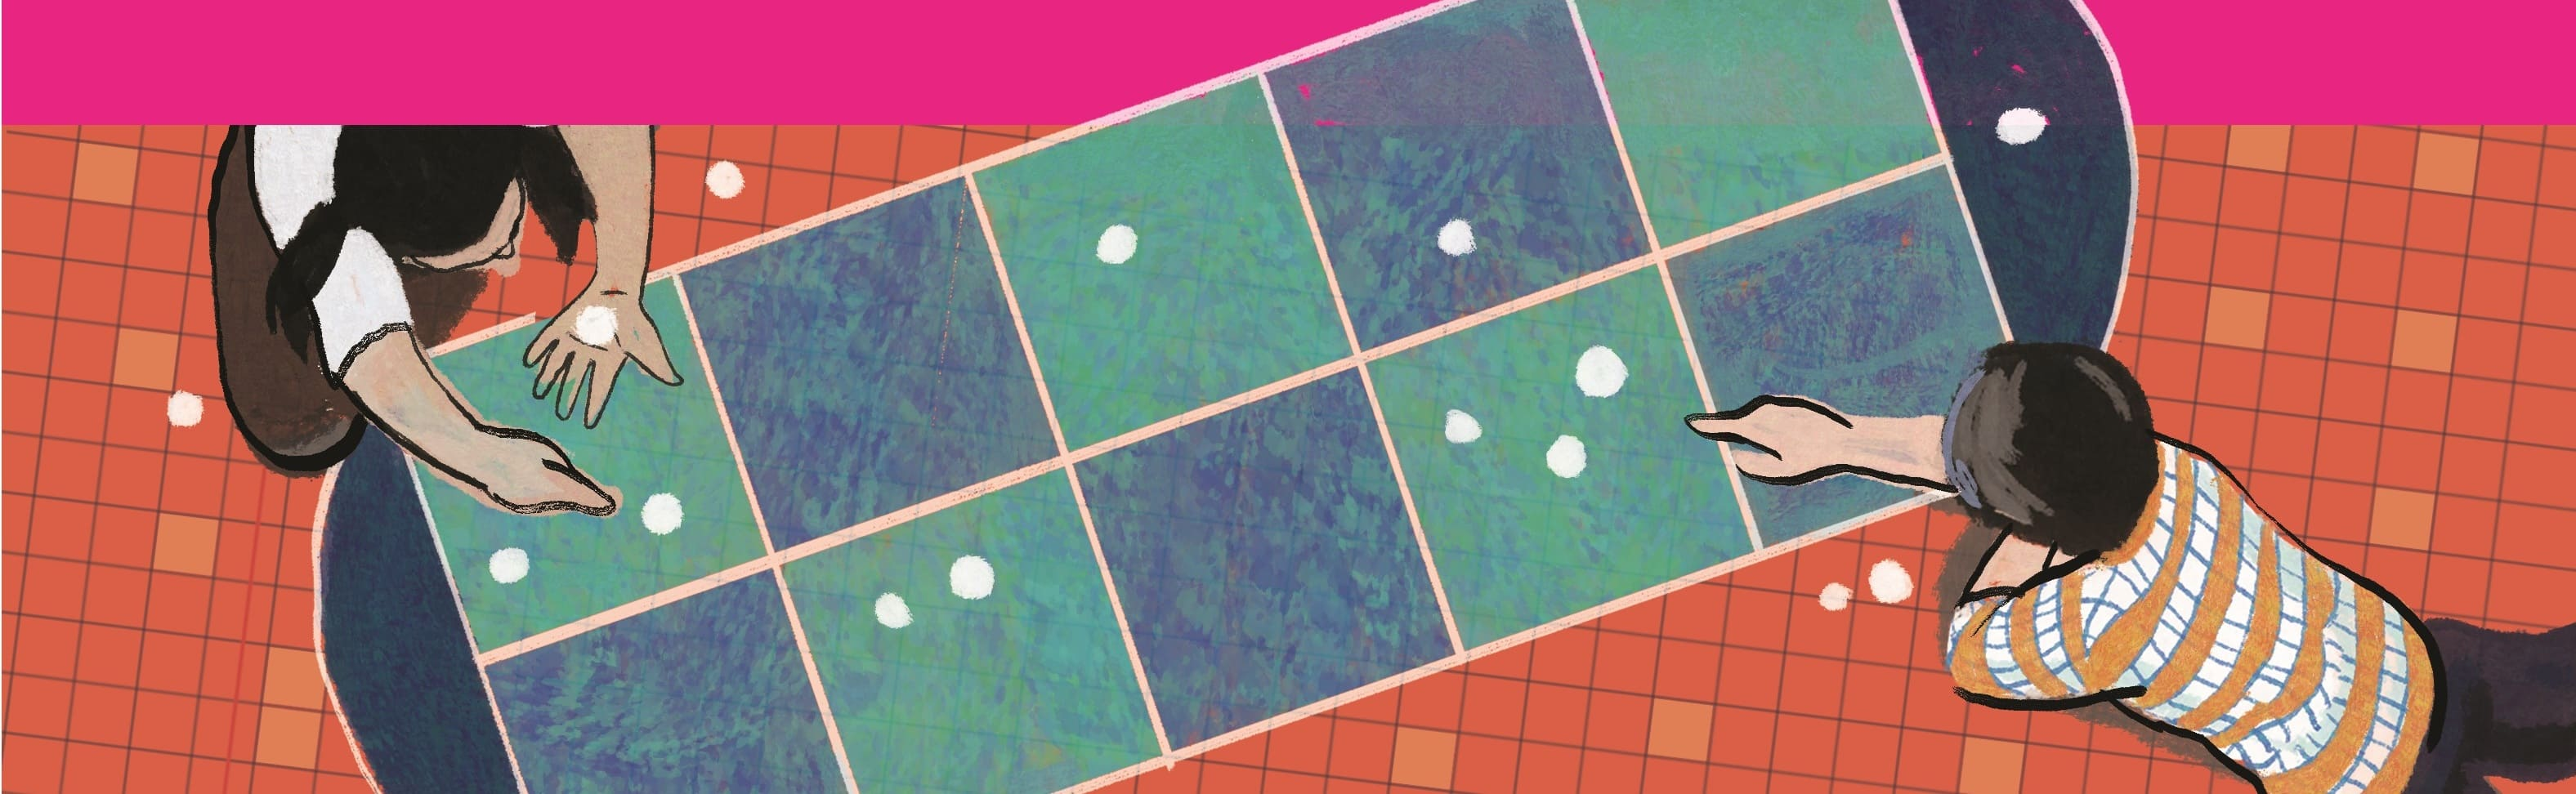
\includegraphics[width=19.3cm]{../bannertoancuabi}}}  
\AddToShipoutPicture*{\put(99,520){
\includegraphics[scale=1]{../tieude1.pdf}}} 
\centering
\endgroup
\vspace*{182pt}

\begin{multicols}{2}
	Tính diện tích của một hình là một chủ đề hay và có nhiều điều thú vị của các bạn nhỏ cuối cấp $1$. Chủ đề này cũng được các thầy cô trong Câu lạc bộ Unicorn Math Circle (UMC) giảng dạy trong nhiều buổi với sự tham gia hào hứng của các bạn học và có nhiều cách giải độc đáo đã được đưa ra. Chúng ta cùng bắt đầu với một dạng tính diện tích trong những bài giảng của các thầy cô -- Tính diện tích hình trên lưới ô vuông. Với cách tính được trình bày trong bài viết này, các bạn nhỏ chưa cần học đến những công thức tính diện tích vẫn có thể làm được nhé, vì chúng ta chỉ dựa vào các ô vuông trên lưới thôi.
	\vskip 0.1cm
	Như nhiều bạn đã biết, lưới ô vuông gồm các đường thẳng song song cách đều nhau theo cả chiều ngang cũng như chiều dọc và tạo thành những hình vuông mà ta quy ước là chiếm $1$ đơn vị diện tích. Dựa vào diện tích của hình vuông đơn vị này chúng ta có thể tính được diện tích của nhiều kiểu hình tạo trên lưới ô vuông.
	\begin{figure}[H]
		\centering
		\vspace*{-5pt}
		\captionsetup{labelformat= empty, justification=centering}
		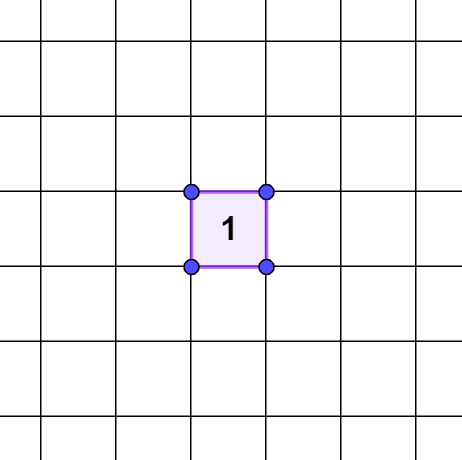
\includegraphics[width=0.48\linewidth]{1}
%		\caption{\small\textit{\color{}.}}
		\vspace*{-2pt}
	\end{figure}
	Trước hết ta bắt đầu với việc tìm diện tích của những hình rất đơn giản nhưng đóng vai trò quan trọng trong việc tính toán diện tích các hình ở các ví dụ sau.
	\vskip 0.1cm
	Hình cơ bản đầu tiên cần tính diện tích là hình chữ nhật có các cạnh nằm trên các đường thẳng của lưới.
	\vskip 0.1cm
	\textbf{\color{toancuabi}Ví dụ} $\pmb{1.}$ Tính diện tích hình chữ nhật được tô đậm trong lưới ô vuông dưới đây.  
	\begin{figure}[H]
		\centering
		\vspace*{-5pt}
		\captionsetup{labelformat= empty, justification=centering}
		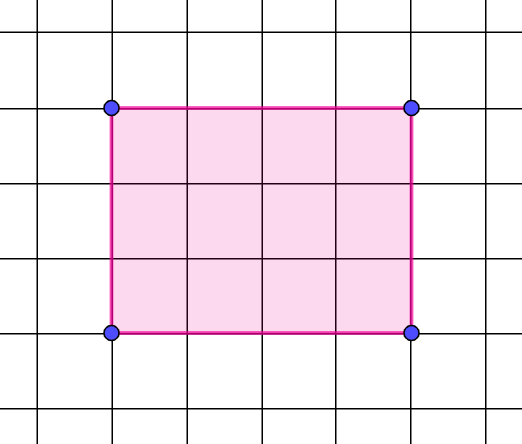
\includegraphics[width=0.55\linewidth]{2}
		%		\caption{\small\textit{\color{}.}}
		\vspace*{-10pt}
	\end{figure}
	\textit{Lời giải.} Bằng cách đếm trực tiếp, ta thấy rằng có tổng cộng $12$ ô vuông được tô đậm, cho nên diện tích phần hình bằng $12$ đơn vị diện tích.
	\vskip 0.1cm
	Các bạn mà học công thức tính diện tích hình chữ nhật rồi sẽ thấy ngay, chiều dài và chiều rộng của hình chữ nhật tương ứng là $4$ và $3$ đơn vị độ dài, từ đó hình chữ nhật có diện tích là: $4 \times 3 = 12$ (đơn vị diện tích).
	\vskip 0.1cm
	Chúng ta tiếp tục với hình cơ bản thứ hai là tam giác có hai cạnh trùng với hai đường dọc và ngang của lưới ô vuông.
	\vskip 0.1cm
	\textbf{\color{toancuabi}Ví dụ} $\pmb{2.}$ Tính diện tích tam giác được tô đậm trong hình dưới đây.
	\begin{figure}[H]
		\centering
		\vspace*{-5pt}
		\captionsetup{labelformat= empty, justification=centering}
		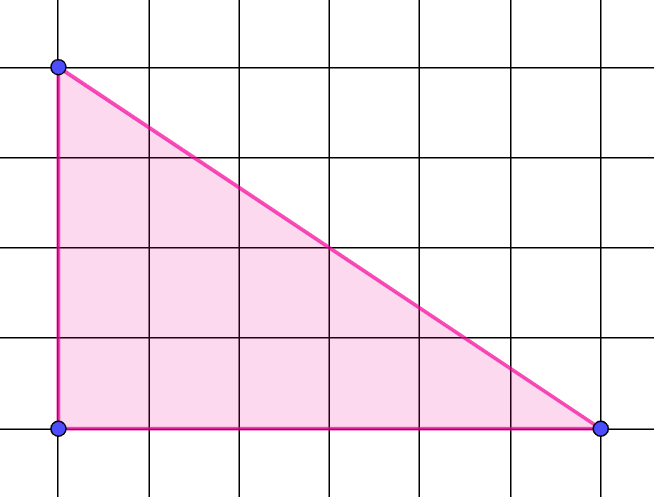
\includegraphics[width=0.55\linewidth]{3}
		%		\caption{\small\textit{\color{}.}}
		\vspace*{-10pt}
	\end{figure}
	\textit{Lời giải.} Ở ví dụ này, các bạn nhỏ quan sát một chút thì sẽ thấy ngay diện tích của tam giác đã cho bằng một nửa hình chữ nhật màu cỡ $6\times4$ được tô màu xanh dương dưới đây.
	\begin{figure}[H]
		\centering
		\vspace*{-5pt}
		\captionsetup{labelformat= empty, justification=centering}
		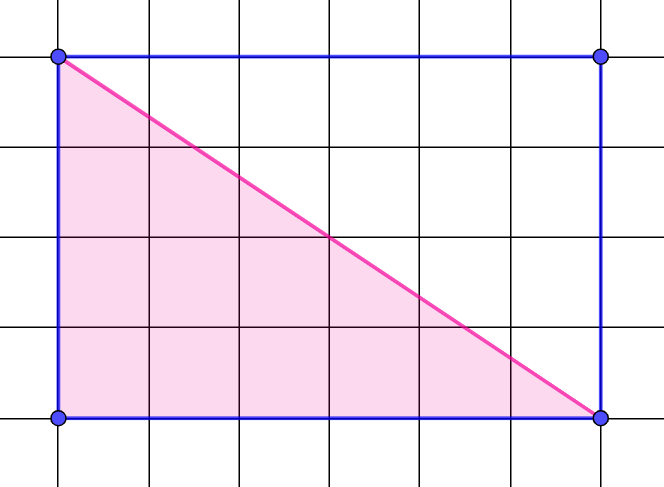
\includegraphics[width=0.55\linewidth]{4}
		%		\caption{\small\textit{\color{}.}}
		\vspace*{-10pt}
	\end{figure}
	Do diện tích hình chữ nhật được tạo bởi $24$ ô vuông nên diện tích hình tam giác bằng $\dfrac{24}{2} =12$ (đơn vị diện tích).
	\vskip 0.1cm
	Ngoài ra, nếu bạn nhỏ nào đã biết công thức tính diện tích tam giác thì tam giác trong Ví dụ $2$ là tam giác vuông với $2$ cạnh góc vuông là $6$ và $4$ đơn vị. Do đó diện tích của tam giác là $d\frac{1}{2}\times 6\times 4 = 12$ đơn vị.
	\vskip 0.1cm
	Hai ví dụ trên cho ta một cái nhìn trực quan về bài toán tính diện tích trên lưới ô vuông, ta chỉ dùng cách đếm đơn thuần số ô vuông trên lưới. Trong các bài toán sau, có thể có nhiều cách giải khác nhau nhưng bài viết đưa ra cách giải mà chỉ dựa vào hai hình cơ bản đã biết cách tính diện tích trong Ví dụ $1$ và Ví dụ $2$.
	\vskip 0.1cm
	Chúng ta lại tiếp tục với tính diện tích của tam giác nhé. Lần này là tam giác chỉ có một cạnh trùng với đường dọc--ngang của lưới và trong trường hợp này, ta không thể áp dụng luôn cách tính như trong Ví dụ $2$. Tuy nhiên bằng cách chia tam giác này thành các tam giác nhỏ có hai cạnh trùng với những đường thẳng của lưới, ta hoàn toàn có thể áp dụng cách tính diện tích tam giác như trong tình huống trên.
	\vskip 0.1cm
	\textbf{\color{toancuabi}Ví dụ} $\pmb{3.}$ Tính diện tích tam giác được tô đậm trong hình cho ở dưới đây.
	\begin{figure}[H]
		\centering
		\vspace*{-5pt}
		\captionsetup{labelformat= empty, justification=centering}
		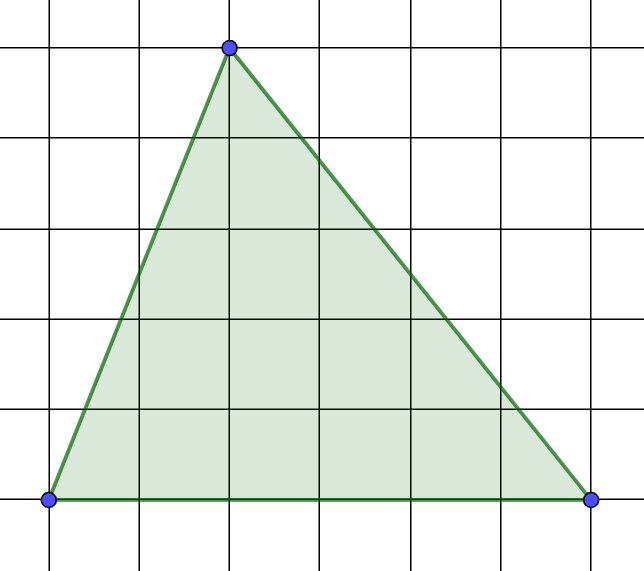
\includegraphics[width=0.55\linewidth]{5}
		%		\caption{\small\textit{\color{}.}}
		\vspace*{-10pt}
	\end{figure}
	\textit{Lời giải.} Ta chia hình tam giác lớn thành hai hình tam giác $(1)$ và $(2)$.
	\begin{figure}[H]
		\centering
		\vspace*{-5pt}
		\captionsetup{labelformat= empty, justification=centering}
		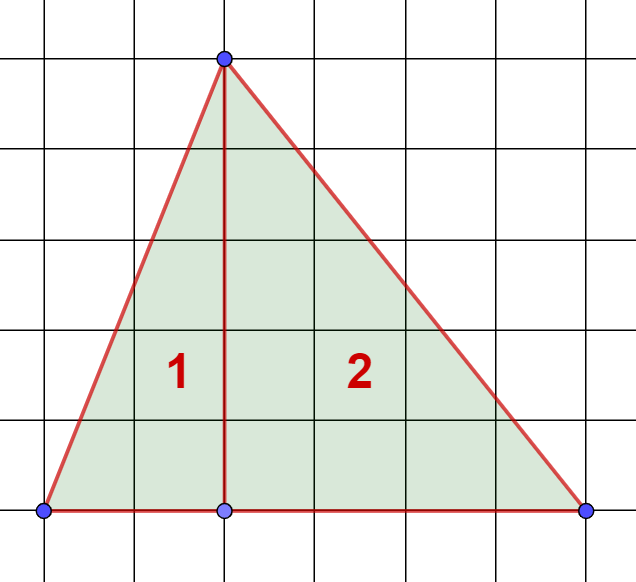
\includegraphics[width=0.55\linewidth]{6}
		%		\caption{\small\textit{\color{}.}}
		\vspace*{-10pt}
	\end{figure}
	Sau đó tính diện tích từng tam giác, tương tự như trong Ví dụ $2$.
	\begin{figure}[H]
		\centering
		\vspace*{-5pt}
		\captionsetup{labelformat= empty, justification=centering}
		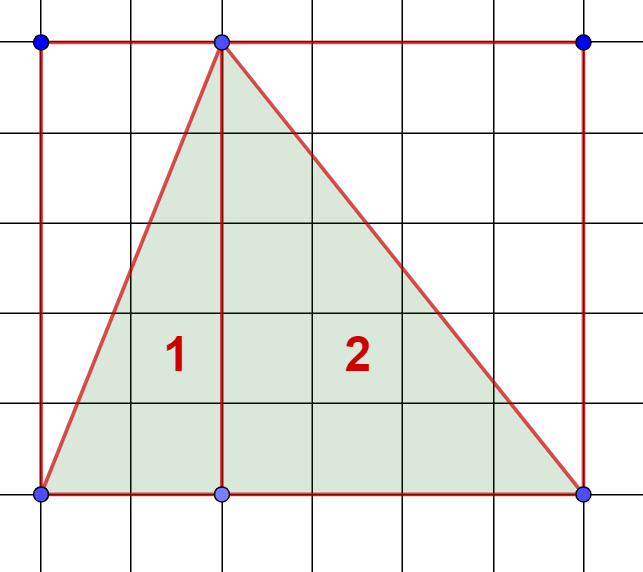
\includegraphics[width=0.55\linewidth]{7}
		%		\caption{\small\textit{\color{}.}}
		\vspace*{-10pt}
	\end{figure}
	Hình tam giác $(1)$ có diện tích bằng một nửa hình chữ nhật bên trái nên có diện tích là: $\dfrac{10}{2}=5$ (đơn vị diện tích).
	\vskip 0.1cm
	Hình tam giác $(2)$ có diện tích bằng một nửa hình chữ nhật bên phải và do đó có diện tích là: $\dfrac{20}{2}=10$ (đơn vị diện tích).
	\vskip 0.1cm
	Suy ra hình cần tính có diện tích bằng $5+10=15$ (đơn vị diện tích). 
	\vskip 0.1cm
	Tính diện tích bằng cách chia hình thành những hình nhỏ hơn không chỉ dừng lại ở việc tính toán những dạng hình học quen thuộc như hình tam giác, hình chữ nhật, ... mà còn có thể áp dụng cho một hình đặc biệt nào đó. Chẳng hạn như hình ``chú mèo" ngộ nghĩnh dưới đây. 
	\vskip 0.1cm 
	\textbf{\color{toancuabi}Ví dụ} $\pmb{4.}$ Tính diện tích ``chú mèo" được cho bởi phần tô đậm trong hình sau.
	\begin{figure}[H]
		\centering
		\vspace*{-5pt}
		\captionsetup{labelformat= empty, justification=centering}
		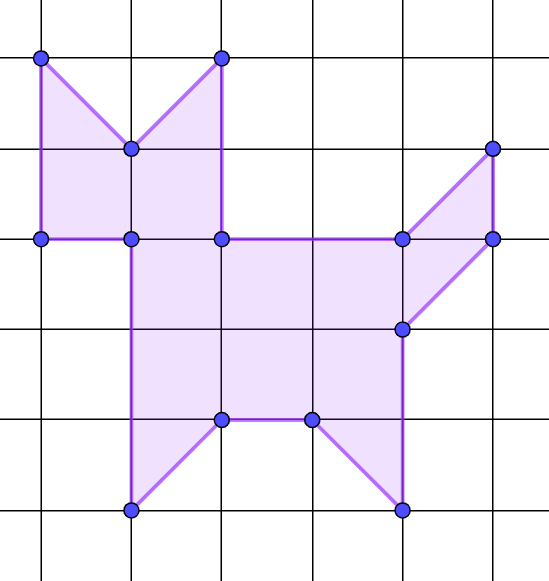
\includegraphics[width=0.5\linewidth]{8}
		%		\caption{\small\textit{\color{}.}}
		\vspace*{-10pt}
	\end{figure}
	\textit{Lời giải.} Ở hình trên có những tam giác nửa, tức là tam giác có diện tích bằng một nửa hình vuông đơn vị và có diện tích là $\dfrac{1}{2}$ đơn vị diện tích. Ta đếm có tổng cộng $8$ hình vuông và $6$ hình tam giác nửa ($2$ tai, $2$ chân và cái đuôi). Vì thế ``chú mèo" có diện tích bằng $8+\dfrac{1}{2}\times6=11$ đơn vị diện tích.
	\vskip 0.1cm
	\textbf{\color{toancuabi}Bài tập} $\pmb{1.}$ Các bạn nhỏ hãy tính diện tích ``chú ngựa" trong hình sau.
	\begin{figure}[H]
		\centering
		\vspace*{-5pt}
		\captionsetup{labelformat= empty, justification=centering}
		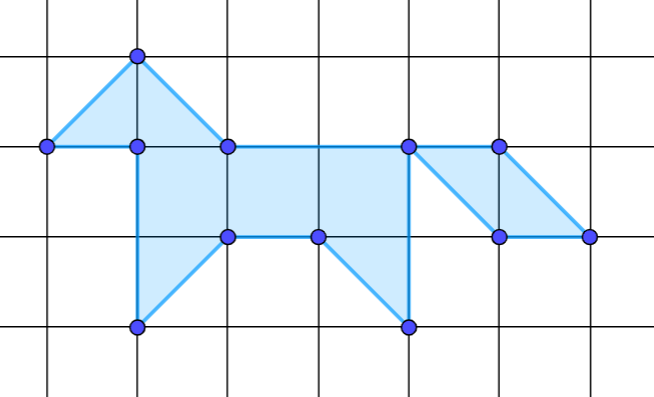
\includegraphics[width=0.58\linewidth]{9}
		%		\caption{\small\textit{\color{}.}}
		\vspace*{-10pt}
	\end{figure}
	Nếu gặp những tình huống hình mà cần tìm diện tích không thể tính trực tiếp bằng việc đếm số ô vuông, hay không thể chia thành những hình cơ bản đã biết cách tính diện tích; chúng ta có thể xem xét cách tìm thông qua phần bù của nó đối với một hình bao quanh. Để đơn giản, phần bù của hình đã cho thường được lấy trong một hình cơ bản đã biết diện tích như hình chữ nhật có các cạnh trùng với những đường thẳng của lưới. Dưới đây là một số ví dụ về những hình chữ nhật thế này.
	\begin{figure}[H]
		\centering
		\vspace*{5pt}
		\captionsetup{labelformat= empty, justification=centering}
		
\includegraphics[width=1\linewidth]{10}
		%		\caption{\small\textit{\color{}.}}
		\vspace*{-15pt}
	\end{figure}
	Diện tích cần tính dưới đây tiếp tục là một tam giác, nhưng lần này là một tam giác tùy ý, không có cạnh nào trùng với những đường thẳng của lưới. 
	\vskip 0.1cm
	\textbf{\color{toancuabi}Ví dụ} $\pmb{5.}$ Tính diện tích của hình được tô đậm sau đây.
	\begin{figure}[H]
		\centering
		\vspace*{-5pt}
		\captionsetup{labelformat= empty, justification=centering}
		
\includegraphics[width=0.5\linewidth]{11}
		%		\caption{\small\textit{\color{}.}}
		\vspace*{-10pt}
	\end{figure}
	\textit{Lời giải.} Rõ ràng với tam giác này, việc tính trực tiếp phần bên trong là khó khăn. Tuy nhiên phần bù của tam giác trong hình chữ nhật bao quanh nó lại là những tam giác như trong Ví dụ $2$ nên ta hoàn toàn có thể tính được ngay.
	\begin{figure}[H]
		\centering
		\vspace*{-5pt}
		\captionsetup{labelformat= empty, justification=centering}
		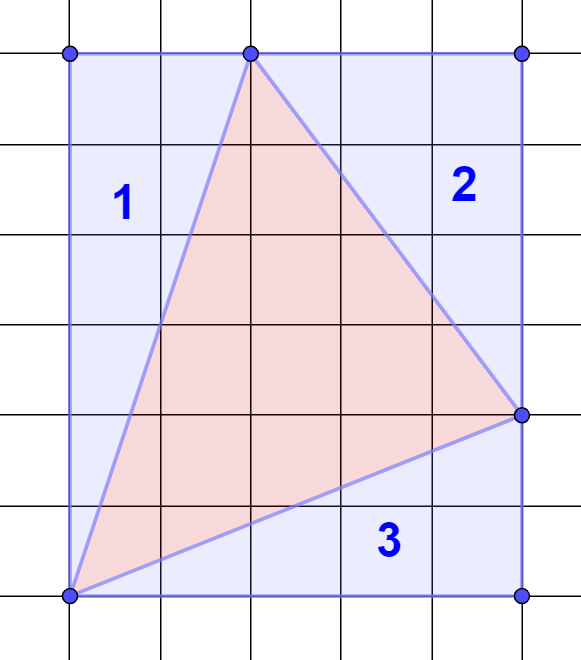
\includegraphics[width=0.5\linewidth]{12}
		%		\caption{\small\textit{\color{}.}}
		\vspace*{-10pt}
	\end{figure}
	Lần lượt gọi ba tam giác phần bù được tô xanh là $(1)$,$(2)$ và $(3)$. Ta thấy
	Hình $(1)$ có diện tích bằng nửa hình chữ nhật cỡ $6\times2$, nên có diện tích bằng $6$.
	\vskip 0.1cm
	Hình $(2)$ có diện tích bằng nửa hình chữ nhật cỡ $4\times3$, nên có diện tích bằng $6$.
	\vskip 0.1cm
	Hình $(3)$ có diện tích bằng nửa hình chữ nhật cỡ $5\times2$, nên có diện tích bằng $5$.
	\vskip 0.1cm
	Vì phần bù được tạo thành bởi ba tam giác vuông $(1)$, $(2)$ và $(3)$ nên diện tích của chúng bằng $6+6+5=17$. Suy ra diện tích tam giác được tô đậm bằng $30-17=13$ đơn vị diện tích.
	\vskip 0.1cm
	Để rèn luyện thêm cách tính diện tích dựa trên phần bù, chúng ta cùng luyện tập tiếp những ví dụ sau nhé. 
	\vskip 0.1cm 
	\textbf{\color{toancuabi}Ví dụ} $\pmb{6.}$ Tính diện tích phần hình được tô đậm dưới đây.
	\begin{figure}[H]
		\centering
		\vspace*{-5pt}
		\captionsetup{labelformat= empty, justification=centering}
		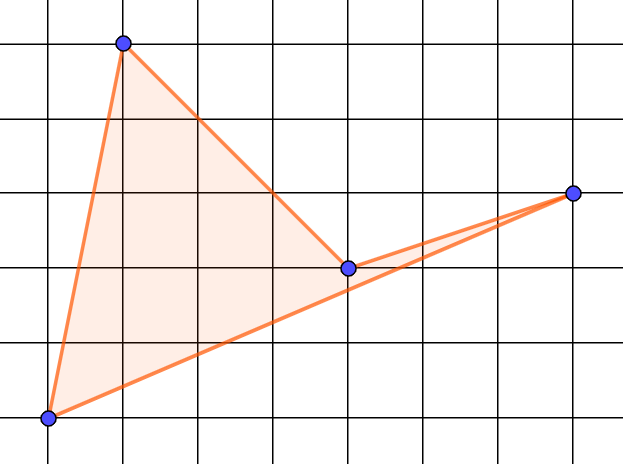
\includegraphics[width=0.6\linewidth]{13}
		%		\caption{\small\textit{\color{}.}}
		\vspace*{-10pt}
	\end{figure}
	\textit{Lời giải.} Trong ví dụ này, ta tiếp tục tính diện tích theo phần bù và chia phần bù của hình đã cho thành các hình quen thuộc đã biết cách tính diện tích. Mỗi bạn nhỏ có thể chọn những cách chia khác nhau, chẳng hạn ta có thể chia đơn giản như sau: 
	\begin{figure}[H]
		\centering
		\vspace*{-5pt}
		\captionsetup{labelformat= empty, justification=centering}
		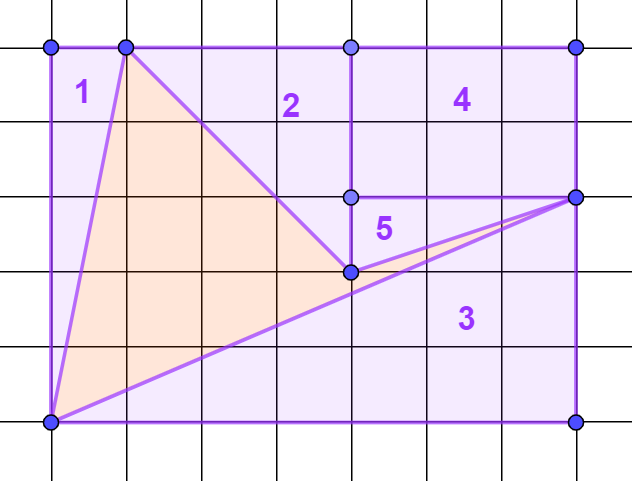
\includegraphics[width=0.6\linewidth]{14}
		%		\caption{\small\textit{\color{}.}}
		\vspace*{-10pt}
	\end{figure}
	Phần bù của hình đã cho được chia thành năm hình $(1)$, $(2)$, $(3)$, $(4)$ và $(5)$. Khi đó
	\vskip 0.1cm
	Hình tam giác $(1)$ có diện tích bằng $\dfrac{1}{2} \times 5=2{,}5$ (đơn vị diện tích)
	\vskip 0.1cm
	Hình tam giác $(2)$ có diện tích bằng $\dfrac{1}{2} \times9 =4{,}5$ (đơn vị diện tích)
	\vskip 0.1cm
	Hình tam giác $(3)$ có diện tích bằng $\dfrac{1}{2} \times 21=10{,}5$ (đơn vị diện tích)
	\vskip 0.1cm
	Hình chữ nhật $(4)$ có diện tích bằng $6$ (đơn vị diện tích)
	\vskip 0.1cm
	Hình tam giác $(5)$ có diện tích bằng $\dfrac{1}{2} \times3=1{,}5$ (đơn vị diện tích)
	\vskip 0.1cm
	Vậy tổng diện tích của chúng bằng $2{,}5+4{,}5+10{,}5+6+1{,}5 =25$. Suy ra diện tích hình tam giác tô đậm bằng $7\times 7-25=24$ đơn vị diện tích. 
	\vskip 0.1cm
	Qua những ví dụ trên, các bạn nhỏ chắc là đã biết các tính qua phần bù rồi đúng không? Bài tập sau để chúng ta luyện tập thêm nhé. 
	\vskip 0.1cm
	\textbf{\color{toancuabi}Bài tập} $\pmb{2.}$ Tính diện tích phần hình được tô đậm trong các hình dưới đây.
	\begin{figure}[H]
		\centering
		\vspace*{-5pt}
		\captionsetup{labelformat= empty, justification=centering}
		
\includegraphics[width=0.55\linewidth]{15}
		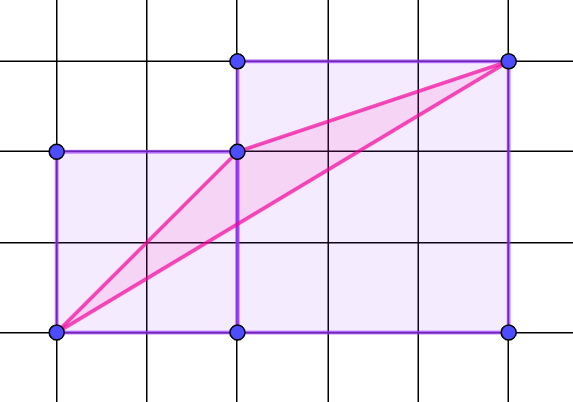
\includegraphics[width=0.48\linewidth]{16}
		%		\caption{\small\textit{\color{}.}}
		\vspace*{-10pt}
	\end{figure}
	Việc tính theo phần bù chỉ hiệu quả khi phần bù được cấu tạo bởi những hình cơ bản như hình chữ nhật, hình tam giác như trong hai ví dụ đầu tiên. Vì thế các bạn nhỏ cần chia thật khéo, sao cho mọi hình đều có dạng quen thuộc nhé!  
	\vskip 0.1cm
	Đôi khi trong quá trình làm bài, có thể các bạn nhỏ sẽ gặp phải tình huống thế này: sau khi đọc xong đề, ta biết chắc rằng bài đó không thể làm theo cách trực tiếp và do đó ta nghĩ tới cách tính theo phần bù. Nhưng mà nếu tính theo phần bù, thậm chí đã có thao tác chia hình, thì cũng chưa chắc tìm ra đáp án ngay được. Lúc này các bạn nhỏ có thể nghĩ tới việc tính những phần bù này bằng cách lấy bù trong một hình khác. Ví dụ sau minh họa diện tích được tính theo cách này.  
	\vskip 0.1cm
	\textbf{\color{toancuabi}Ví dụ} $\pmb{7.}$ Tính diện tích phần hình được tô đậm (AFHI) trong hình dưới đây
	\begin{figure}[H]
		\centering
%		\vspace*{-5pt}
		\captionsetup{labelformat= empty, justification=centering}
		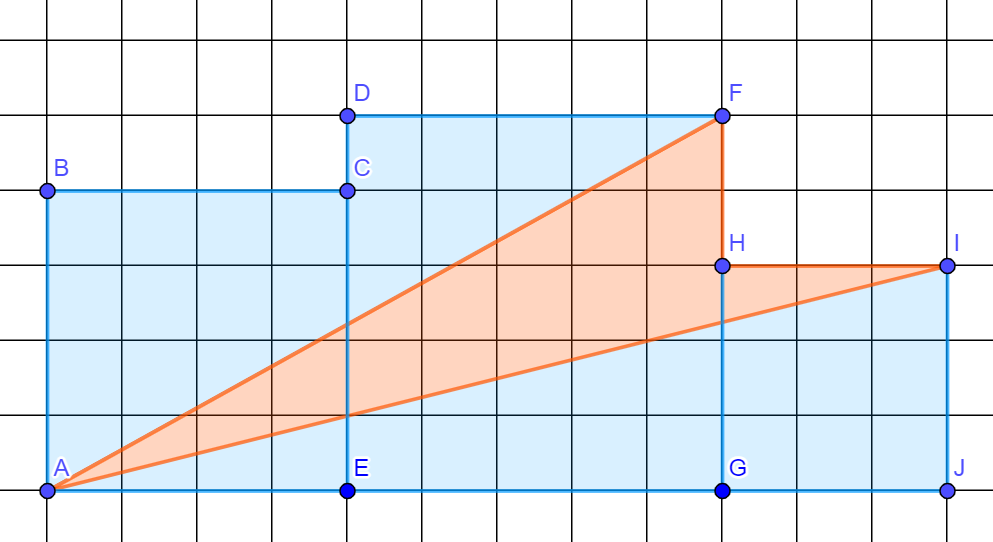
\includegraphics[width=1\linewidth]{17}
		%		\caption{\small\textit{\color{}.}}
		\vspace*{-15pt}
	\end{figure}
	\textit{Lời giải.} Việc tính toán trực tiếp là không dễ dàng trong trường hợp này, do đó ta thử tính theo cách lấy phần bù nhé. Ta bao hình đã cho bởi đa giác $AJIHFDCB$, là ghép của ba hình vuông $ABCE$, $EDFG$ và $GHIJ$. Khi đó phần bù của đa giác $AFHI$ là tam giác $AIJ$ và đa giác $ABCDF$.
	\vskip 0.1cm
	Các bạn nhỏ dễ dàng tính được diện tích tam giác $AIJ$, nhưng với đa giác $ABCDF$ thì tính như thế nào nhỉ? 
	\vskip 0.1cm
	Trước hết, ta có ngay diện tích tam giác $AIJ$ bằng một nửa hình chữ nhật cỡ $12\times3$, nên có diện tích là: $\dfrac{1}{2}\times 36=18$ (đơn vị diện tích). 
	\begin{figure}[H]
		\centering
%		\vspace*{-5pt}
		\captionsetup{labelformat= empty, justification=centering}
		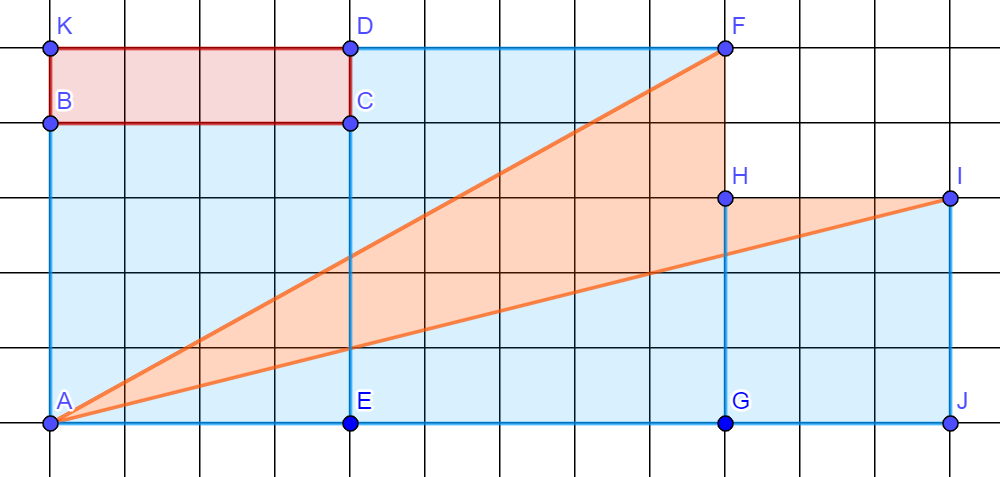
\includegraphics[width=1\linewidth]{18}
		%		\caption{\small\textit{\color{}.}}
		\vspace*{-15pt}
	\end{figure}
	Tiếp theo là xét tới đa giác $ABCDF$. Mặc dù có thể tính trực tiếp bằng cách chia đa giác thành $3$ tam giác $ABC$, $CDF$ và $ACF$, tuy nhiên việc tìm diện tích tam $ACF$ tương đối dài! Để ý kỹ một chút các bạn nhỏ sẽ thấy rằng nếu lấy đa giác $ABCDF$ ghép với hình chữ nhật $BKDC$ ở góc trên cùng bên trái, thì sẽ thu được tam giác vuông $AKF$ có diện tích bằng một nửa hình chữ nhật cỡ $9\times5$; hay nói cách khác, ta đang đi tính diện tích phần bù theo một phần bù khác. 
	\vskip 0.1cm
	Từ hình vẽ ta có nhận xét rằng, 
	\begin{align*}
		S_{AKF}=S_{ABCDF}+S_{BKDC},
	\end{align*} 
	Suy ra diện tích đa giác $ABCDF$ bằng  $\dfrac{1}{2} \times45-4=18{,}5$ (đơn vị diện tích). 
	\vskip 0.1cm
	Như vậy $S_{AFHI}=50-S_{ABCDF}-S_{AIJ}=50-18{,}5-18=13{,}5$ (đơn vị diện tích). 
	\vskip 0.1cm
	Ngoài cách làm ở trên ra thì các bạn nhỏ có thể nhìn nhận bài toán theo hướng khác như sau:  đa giác $AFHI$ thực chất nằm trong hình chữ nhật $AKLJ$, khi đó phần bù gồm tam giác $AKF$, hình chữ nhật $FLIH$ và tam giác $AIJ$. 
	\begin{figure}[H]
		\centering
%		\vspace*{-5pt}
		\captionsetup{labelformat= empty, justification=centering}
		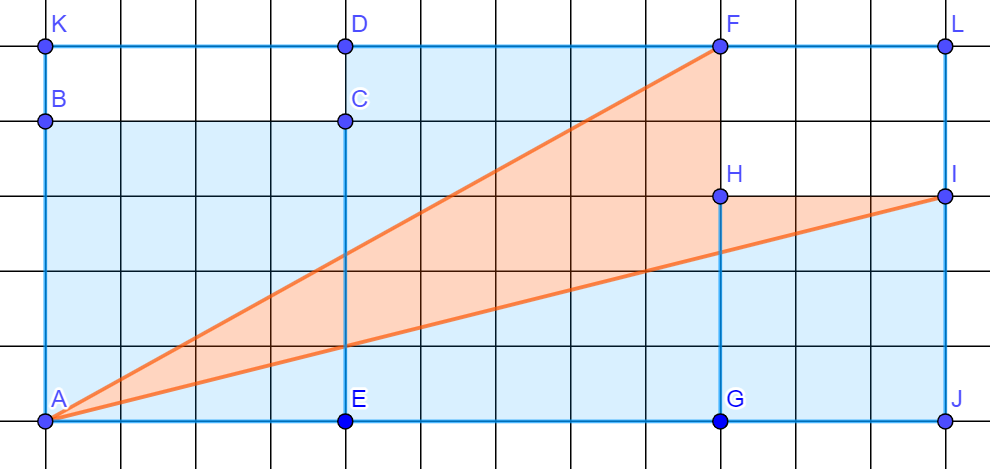
\includegraphics[width=1\linewidth]{19}
		%		\caption{\small\textit{\color{}.}}
		\vspace*{-15pt}
	\end{figure}
	Vậy diện tích đa giác $AFHI$ bằng 
	\begin{align*}
		S_{AFHI}&=S_{AKLJ}-S_{FLIH}-S_{AKF}-S_{AIJ}\\ 
		&=12\times5-6-22{,}5-18\\
		&=13{,}5 \text{ (đơn vị diện tích)}.
	\end{align*}
	Từ Ví dụ $7$ ta thấy rằng việc tính diện tích bằng phần bù có rất nhiều cách làm khác nhau, chủ yếu phụ thuộc vào cách nhìn hình học của từng bạn.   
	\vskip 0.1cm
	Bài tập sau để các em luyện tập thêm nhé.
	\vskip 0.1cm
	\textbf{\color{toancuabi}Bài tập} $\pmb{3.}$ Tính diện tích các phần hình được tô đậm dưới đây.
		\begin{figure}[H]
		\centering
		\vspace*{-5pt}
		\captionsetup{labelformat= empty, justification=centering}
		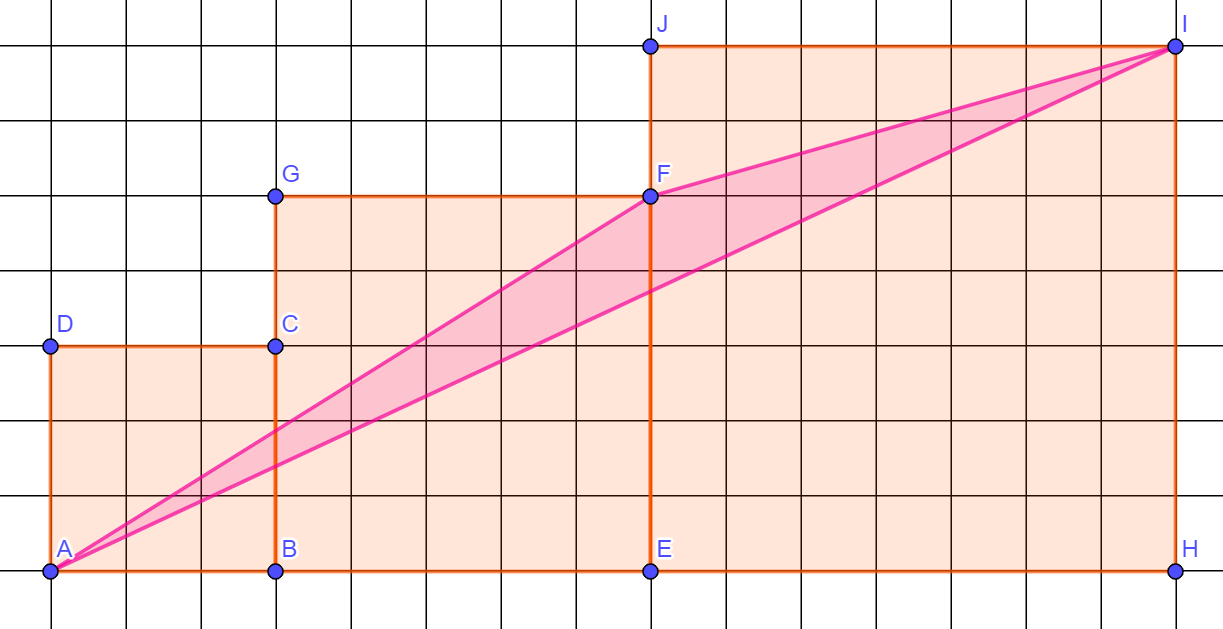
\includegraphics[width=1\linewidth]{20}
		%		\caption{\small\textit{\color{}.}}
		\vspace*{-15pt}
	\end{figure}
\begin{figure}[H]
	\centering
	\vspace*{5pt}
	\captionsetup{labelformat= empty, justification=centering}
	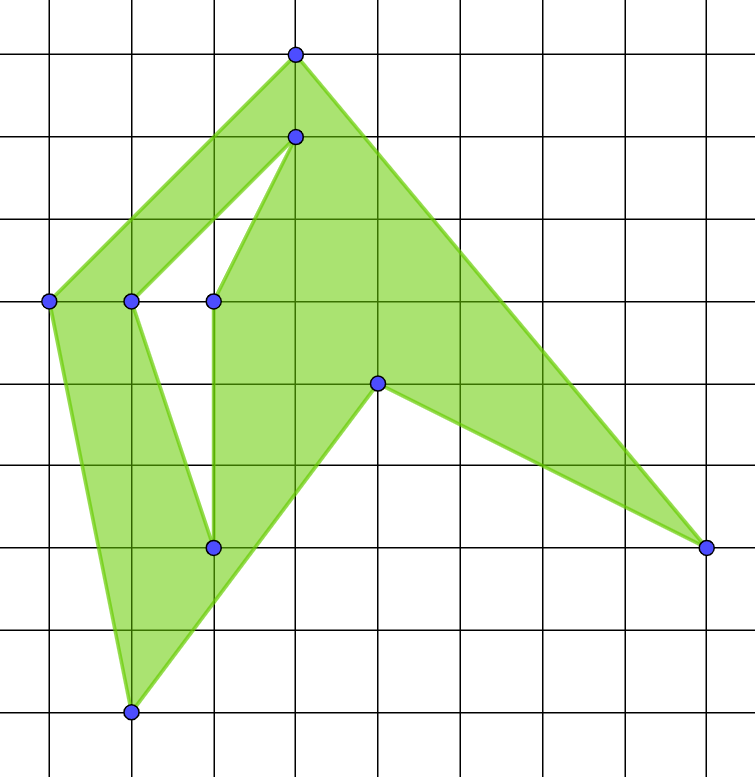
\includegraphics[width=0.58\linewidth]{21}
	%		\caption{\small\textit{\color{}.}}
	\vspace*{-10pt}
\end{figure}
	Vậy là chúng ta đã cùng nhau tìm hiểu về một số phương pháp thường sử dụng khi làm bài toán tính diện tích trên lưới kẻ ô vuông. Tuy rằng tư tưởng của mỗi phương pháp không quá khó hiểu, nhưng các bạn nhỏ vẫn cần luyện tập thường xuyên để có được phản xạ nhanh nhất khi làm bài nhé. Trên thực tế rất nhiều phương pháp độc đáo khác nữa mà bài viết chưa đề cập tới, bạn nhỏ nào hứng thú với dạng bài này có thể tự tìm hiểu thêm, chắc chắn sẽ rất thú vị đấy! Hẹn gặp lại các em trong những chủ đề tiếp theo của câu lạc bộ Unicorn Math Circle.
\end{multicols}
\vspace*{-10pt}
\rule{1\linewidth}{0.1pt}
\begingroup
\AddToShipoutPicture*{\put(130,485){
\includegraphics[scale=1]{../tieude.pdf}}} 
\centering
\endgroup
\vspace*{48pt}
\begin{multicols}{2}
	Thám tử Xuân Phong cùng vợ là bà Xuân Bích tham gia một buổi dã ngoại cùng với hai cặp vợ chồng khác. Cả hai ông chồng là các nhà báo nổi tiếng, còn các bà vợ của họ cũng đều là các quý bà danh giá trong thành phố. Kết thúc buổi dã ngoại, cả ba cặp vợ chồng cùng quay trở về nhà và ra tới một con sông và họ phải chèo trên một chiếc thuyền nhỏ để vượt qua sông. Thuyền chỉ có thể chở được một lúc đồng thời hai người, và hơn nữa không có một phụ nữ nào trong họ lại biết chèo thuyền.
	\begin{figure}[H]
		\centering
		\vspace*{-5pt}
		\captionsetup{labelformat= empty, justification=centering}
		\includegraphics[width=1\linewidth]{xuanphong}
		\vspace*{-15pt}
	\end{figure}
	Bỗng dưng, đang lúc hào hứng ôn kể lại các câu chuyện điều tra phá án của mình, thám tử Xuân Phong đâm ra xích mích, giận mặt đỏ tía tai với hai nhà báo kia về phương pháp điều tra đặc biệt thông minh của mình. Thấy tình hình trở nên căng thẳng như vậy, bà Xuân Bích cũng quyết định đứng về phía chồng mình và không thèm nói chuyện với hai quý bà kia cho bõ tức. còn hai quý bà thì ra sức can ngăn hai ông chồng nóng tính của mình và vẫn giữ hoà khí với thám tử Xuân Phong đáng kính.
	\vskip 0.1cm
	Vậy em có thể giúp Xuân Phong và mọi người tìm ra cách để tất cả các thành viên tham gia buổi dã ngoại đều có thể vượt qua sông, sao cho hai người đang giận dỗi nhau thì không ngồi trên thuyền cùng một lúc, và cũng không đứng đồng thời trên cùng một bờ sông. Và một yêu cầu đặc biệt đặt ra nữa là không một nhà báo nào có thể ở lại một mình trên bất kỳ bờ sông nào cùng với hai quý bà mà không có chồng của bà kia. 
	\vskip 0.1cm
	Bài đố này không khó nhưng rất ít, chỉ khoảng $1$ người trong số $1000$ người tham gia giải, mới có thể giải được ra đáp số mà lại không phải dùng đến giấy và bút đấy các em~ạ!
	
\end{multicols}
\newpage
\begingroup
\AddToShipoutPicture*{\put(112,672){
\includegraphics[scale=1]{../tieude11.pdf}}} 
\centering
\endgroup
\vspace*{35pt}

\begin{multicols}{2}
	$\pmb{1.}$ Một chiếc tàu cao tốc dài $18$ m đi ngang qua một cột cây số trong vòng $9$ giây. Hỏi chiếc tàu đó cần bao nhiêu thời gian để đi qua hết một cây cầu dài $36$ m. 
	\begin{figure}[H]
		\centering
		\vspace*{-10pt}
		\captionsetup{labelformat= empty, justification=centering}
		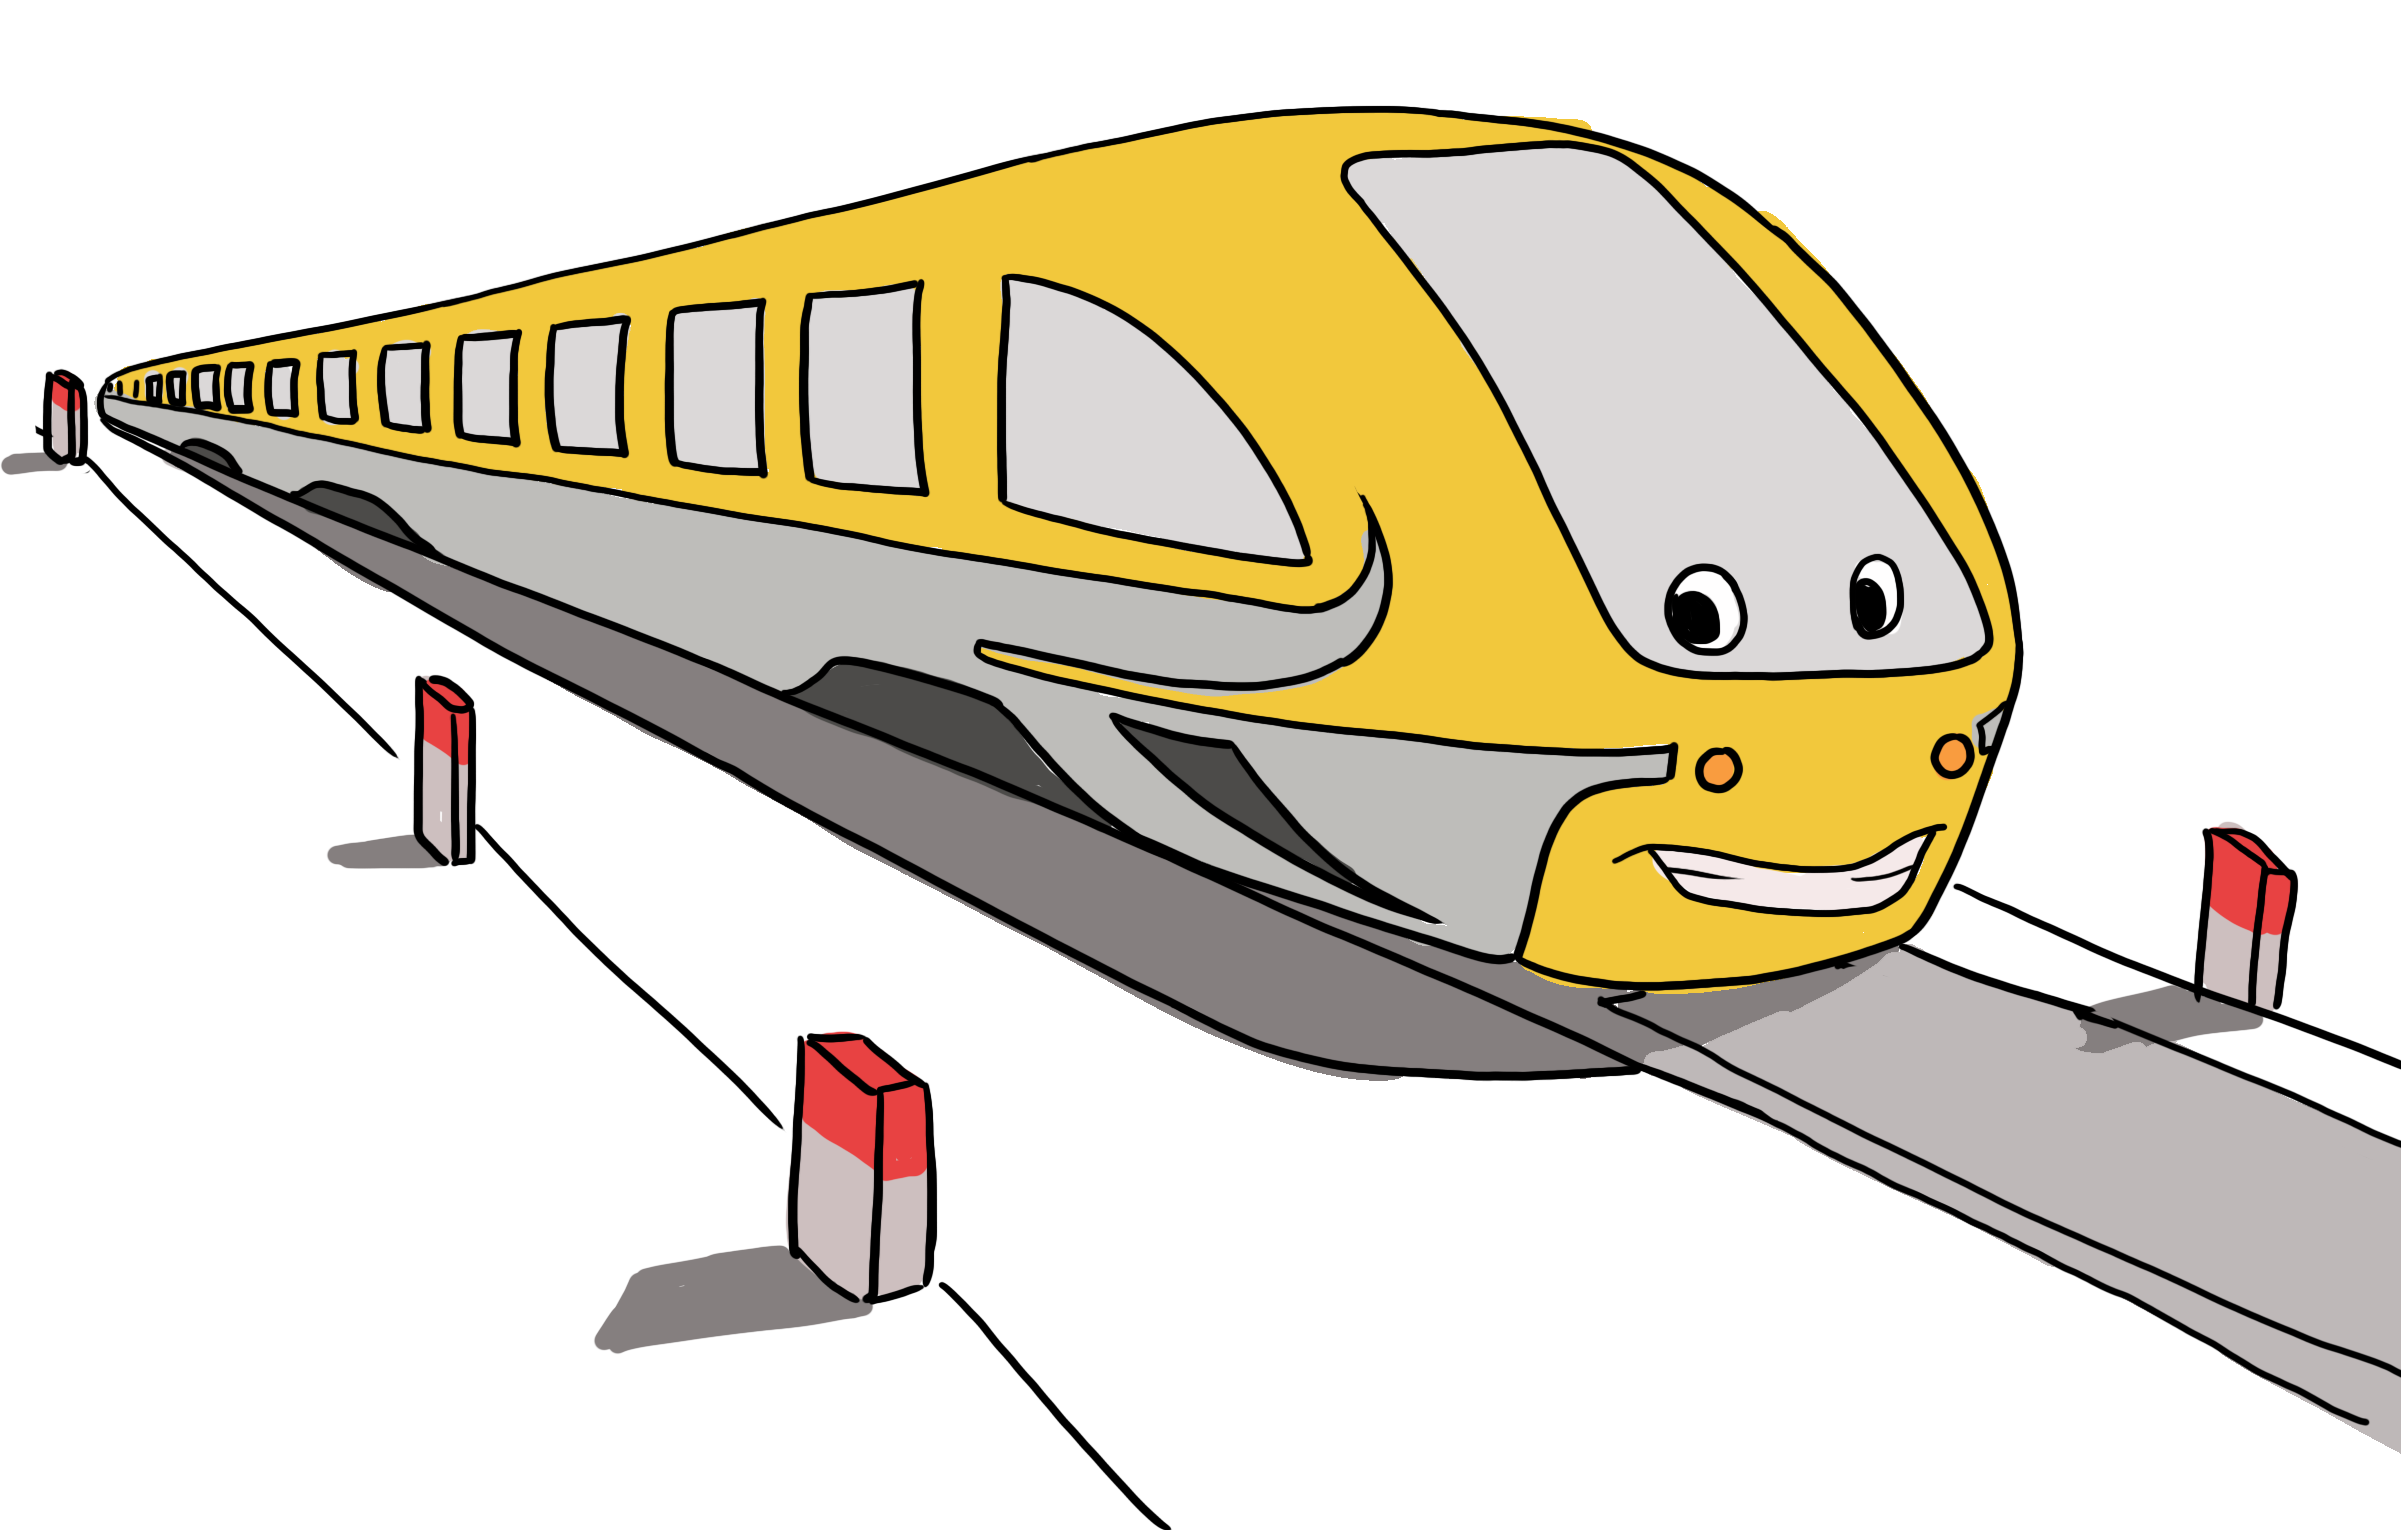
\includegraphics[width=1\linewidth]{Pi10_ToanBi_Bai1}
		\vspace*{-15pt}
	\end{figure}
	\vskip 0.1cm
	$\pmb{2.}$ Hai cậu bé đi bán cam để gây quỹ xây dựng thư viện. Mỗi cậu có $30$ quả cam. Cậu thứ nhất bán  $10{.}000$ đồng hai quả cam, cậu thứ hai bán $10{.}000$ đồng ba quả cam. Trong lúc đang chuẩn bị bày cam ra bán thì một cậu bị gọi về nhà nên cậu ta nhờ cậu thứ hai bán hộ số cam của mình. Tất cả số cam còn lại được cậu bé thứ hai bán với giá $20{.}000$ đồng năm quả. Nếu như số cam bán riêng như dự định lúc đầu thì đã thu được là $150{.}000$ đồng và $100{.}000$ đồng, tức là tổng cộng có $250{.}000$ đồng, nhưng vì bán gộp $20{.}000$ đồng cho $5$ quả nên  hai cậu chỉ thu được $240{.}000$ đồng. Hỏi số tiền bị hụt $10{.}000$ đồng đã mất ở chỗ nào?
	\begin{figure}[H]
		\centering
		\vspace*{-10pt}
		\captionsetup{labelformat= empty, justification=centering}
		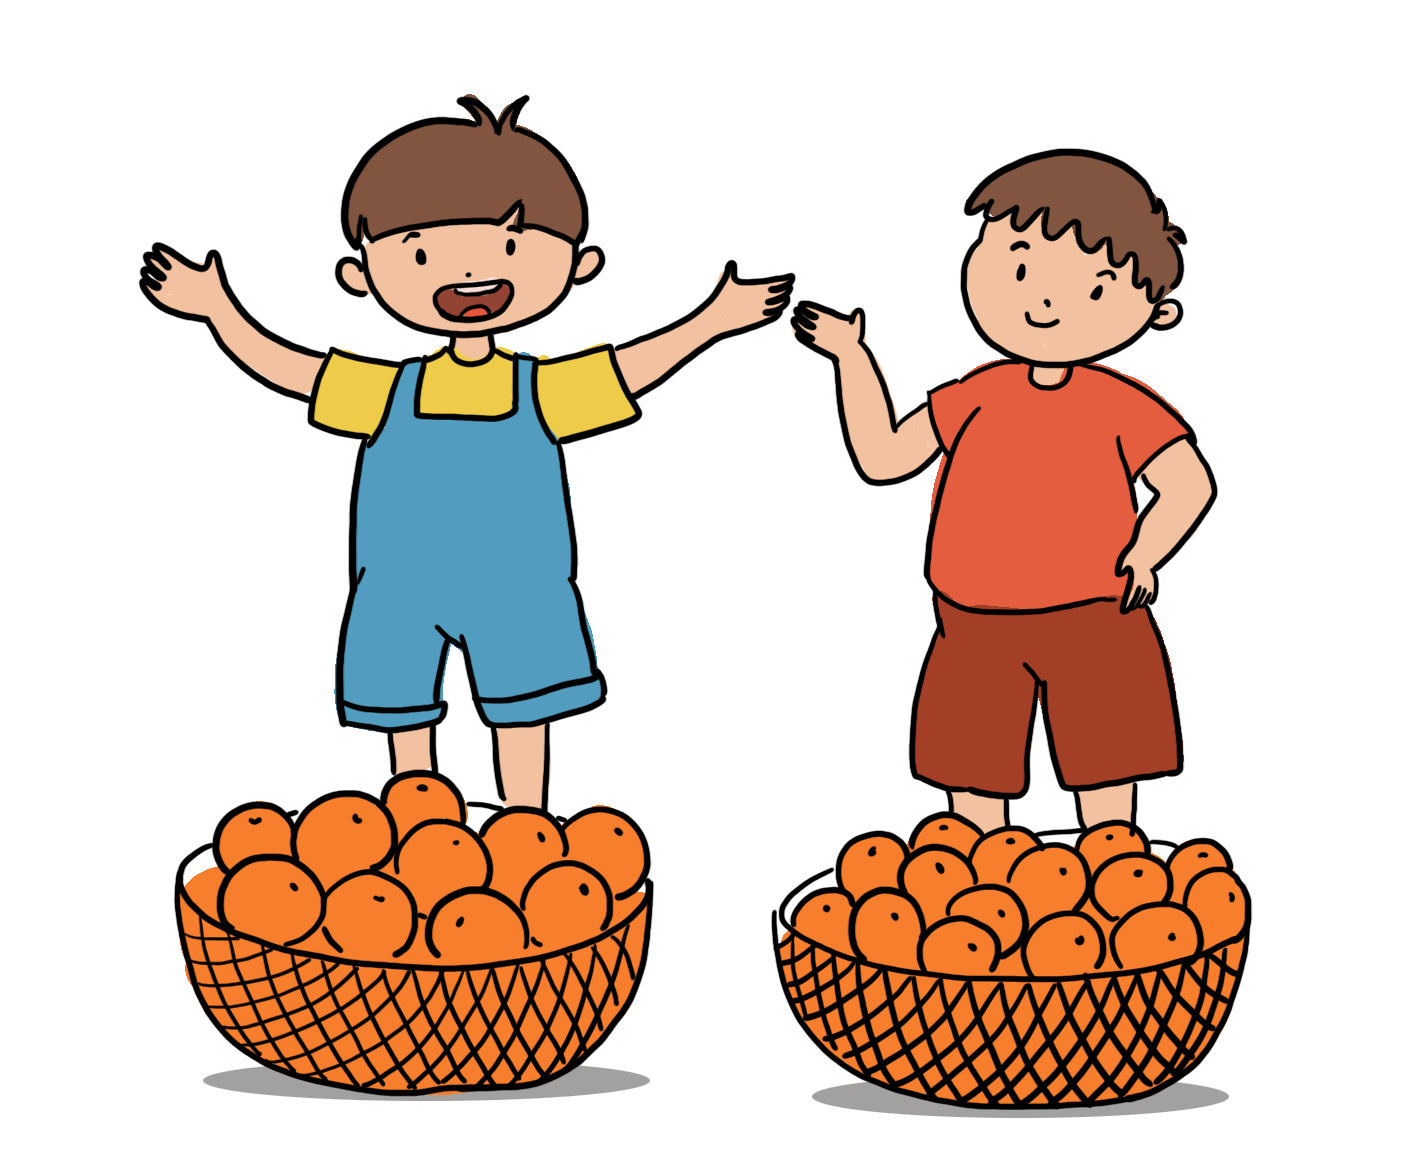
\includegraphics[width=0.8\linewidth]{Pi10_ToanBi_Bai2}
		\vspace*{-10pt}
	\end{figure}
	\vskip 0.1cm
	$\pmb{3.}$ Có ba người bạn tập trung lại để đi cắm trại và họ chỉ có duy nhất một chiếc xe máy có $2$ chỗ ngồi. Liệu họ có thể vượt được quãng đường dài $60$ km tới nơi cắm trại sau khoảng thời gian $3$ giờ đồng hồ được hay không, biết rằng vận tốc của mỗi người đi bộ là $5$ km/giờ và vận tốc của xe máy (có tải hay không có tải) luôn là $50$ km/giờ?
	\begin{figure}[H]
		\centering
		\vspace*{-5pt}
		\captionsetup{labelformat= empty, justification=centering}
		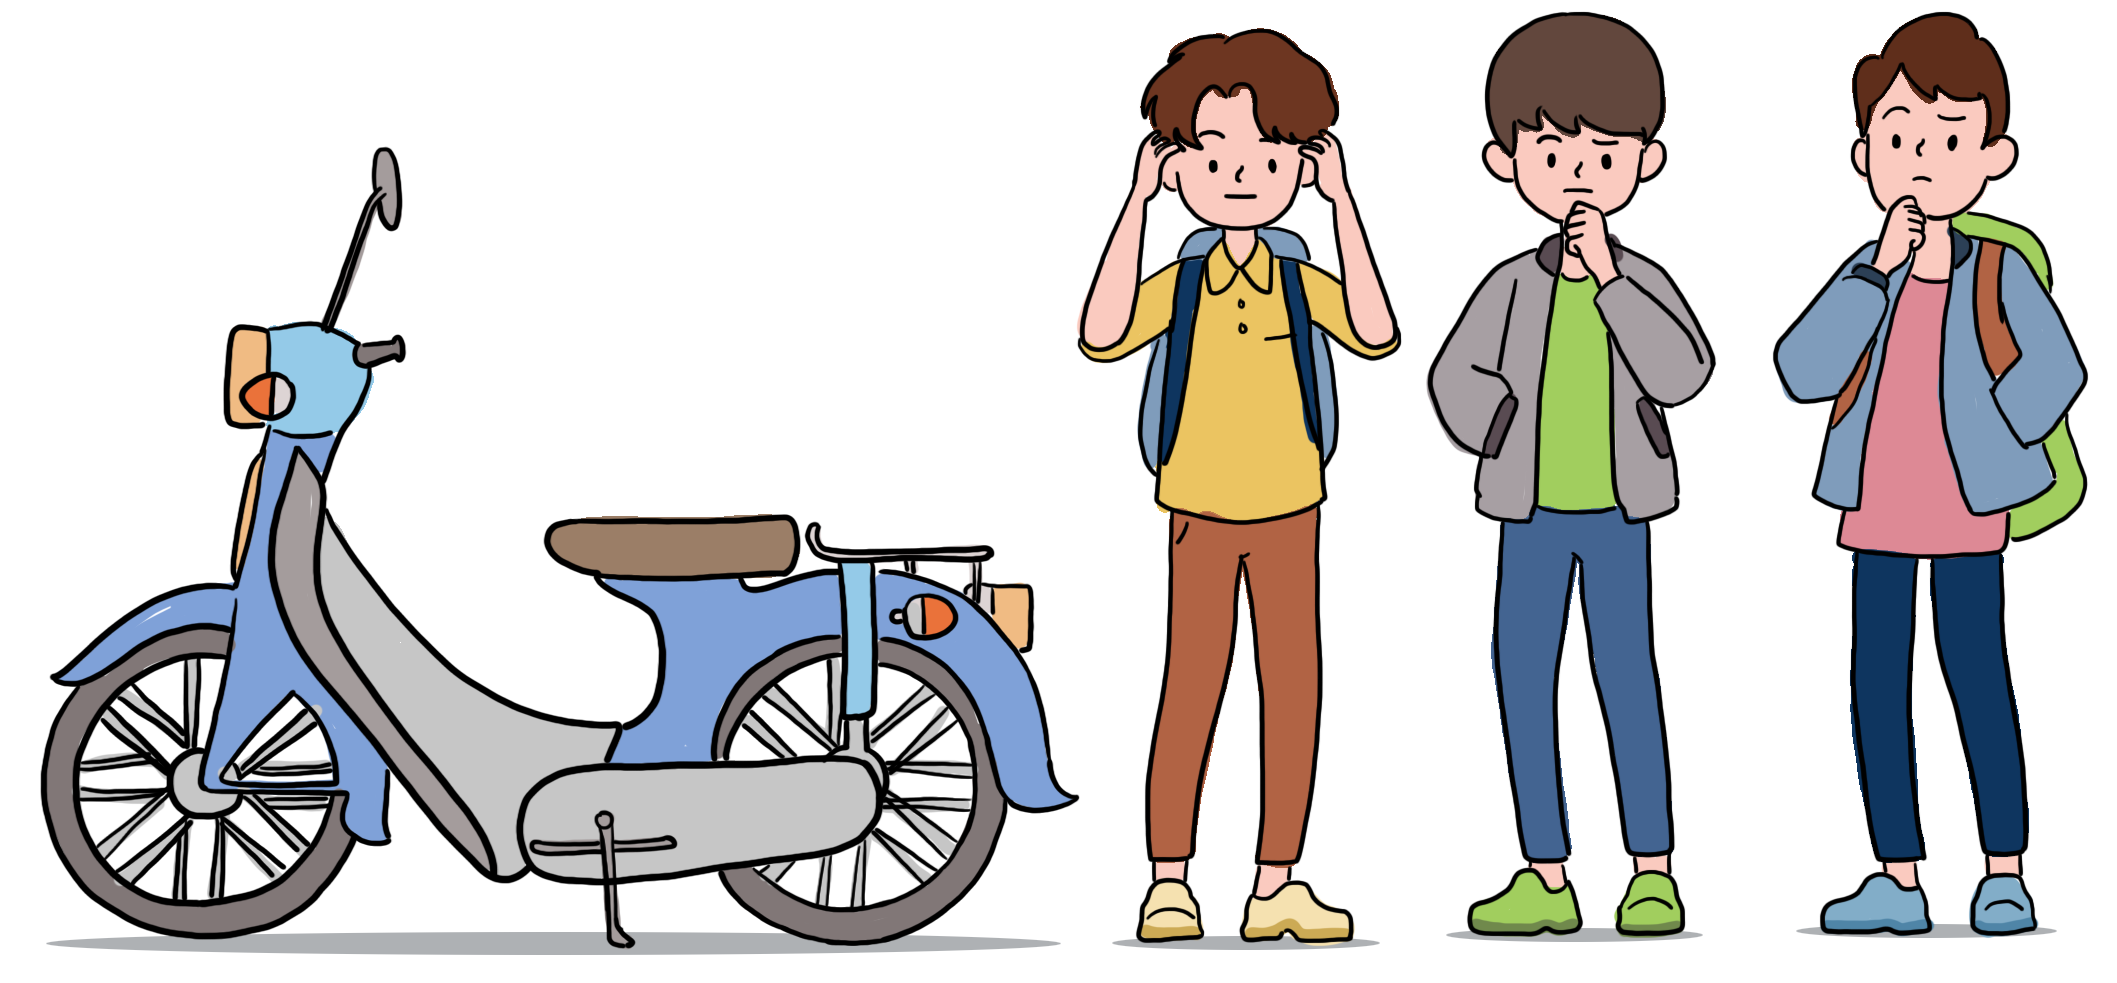
\includegraphics[width=1\linewidth]{Pi10_ToanBi_Bai3}
		\vspace*{-15pt}
	\end{figure}
	$\pmb{4.}$ Có $100$ chiếc thẻ bài bằng nhựa đánh số từ $1$ tới $100$ lần lượt được xếp thành hàng ngang. Cứ hai chiếc thẻ xếp cách nhau một chiếc thẻ khác đều có thể đổi chỗ được cho nhau. Liệu em có thể đổi chỗ các chiếc thẻ này bằng cách như trên để xếp lại được $100$ chiếc thẻ trên theo thứ tự ngược lại được hay không?
	\begin{figure}[H]
		\centering
		\vspace*{-5pt}
		\captionsetup{labelformat= empty, justification=centering}
		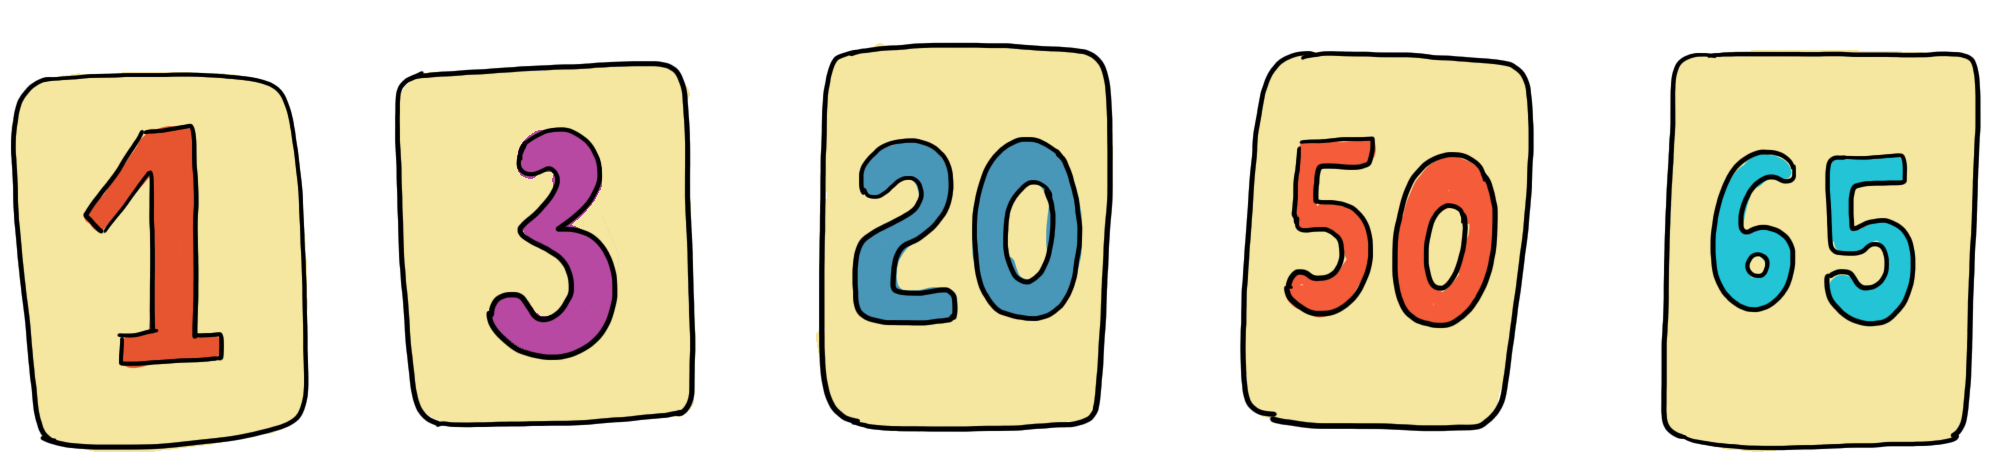
\includegraphics[width=1\linewidth]{Pi10_ToanBi_Bai4}
		\vspace*{-15pt}
	\end{figure}
	$\pmb{5.}$ Trong ngày khai giảng các bạn học sinh gặp lại nhau sau một mùa hè nên vô cùng mừng rỡ. Gặp lại bạn bè cũ và ai cũng tranh thủ bắt tay bạn mình. Kết thúc màn chào hỏi vui tươi sôi nổi, anh phụ trách thống kê lại trong cuốn sổ tổng số bạn học sinh đã có số lẻ lần bắt tay: tổng cộng là $67$ bạn. Bạn Lâm đứng cạnh anh phụ trách nói nhỏ ``Anh ơi, anh đếm nhầm rồi, chắc chắn không phải là $67$ bạn ạ". Anh phụ trách vô cùng ngạc nhiên, vì sao Lâm lại biết vậy. Em có thể giải thích vì sao Lâm lại cho rằng anh phụ trách đếm nhầm được không?
	\begin{figure}[H]
		\centering
%		\vspace*{-5pt}
		\captionsetup{labelformat= empty, justification=centering}
		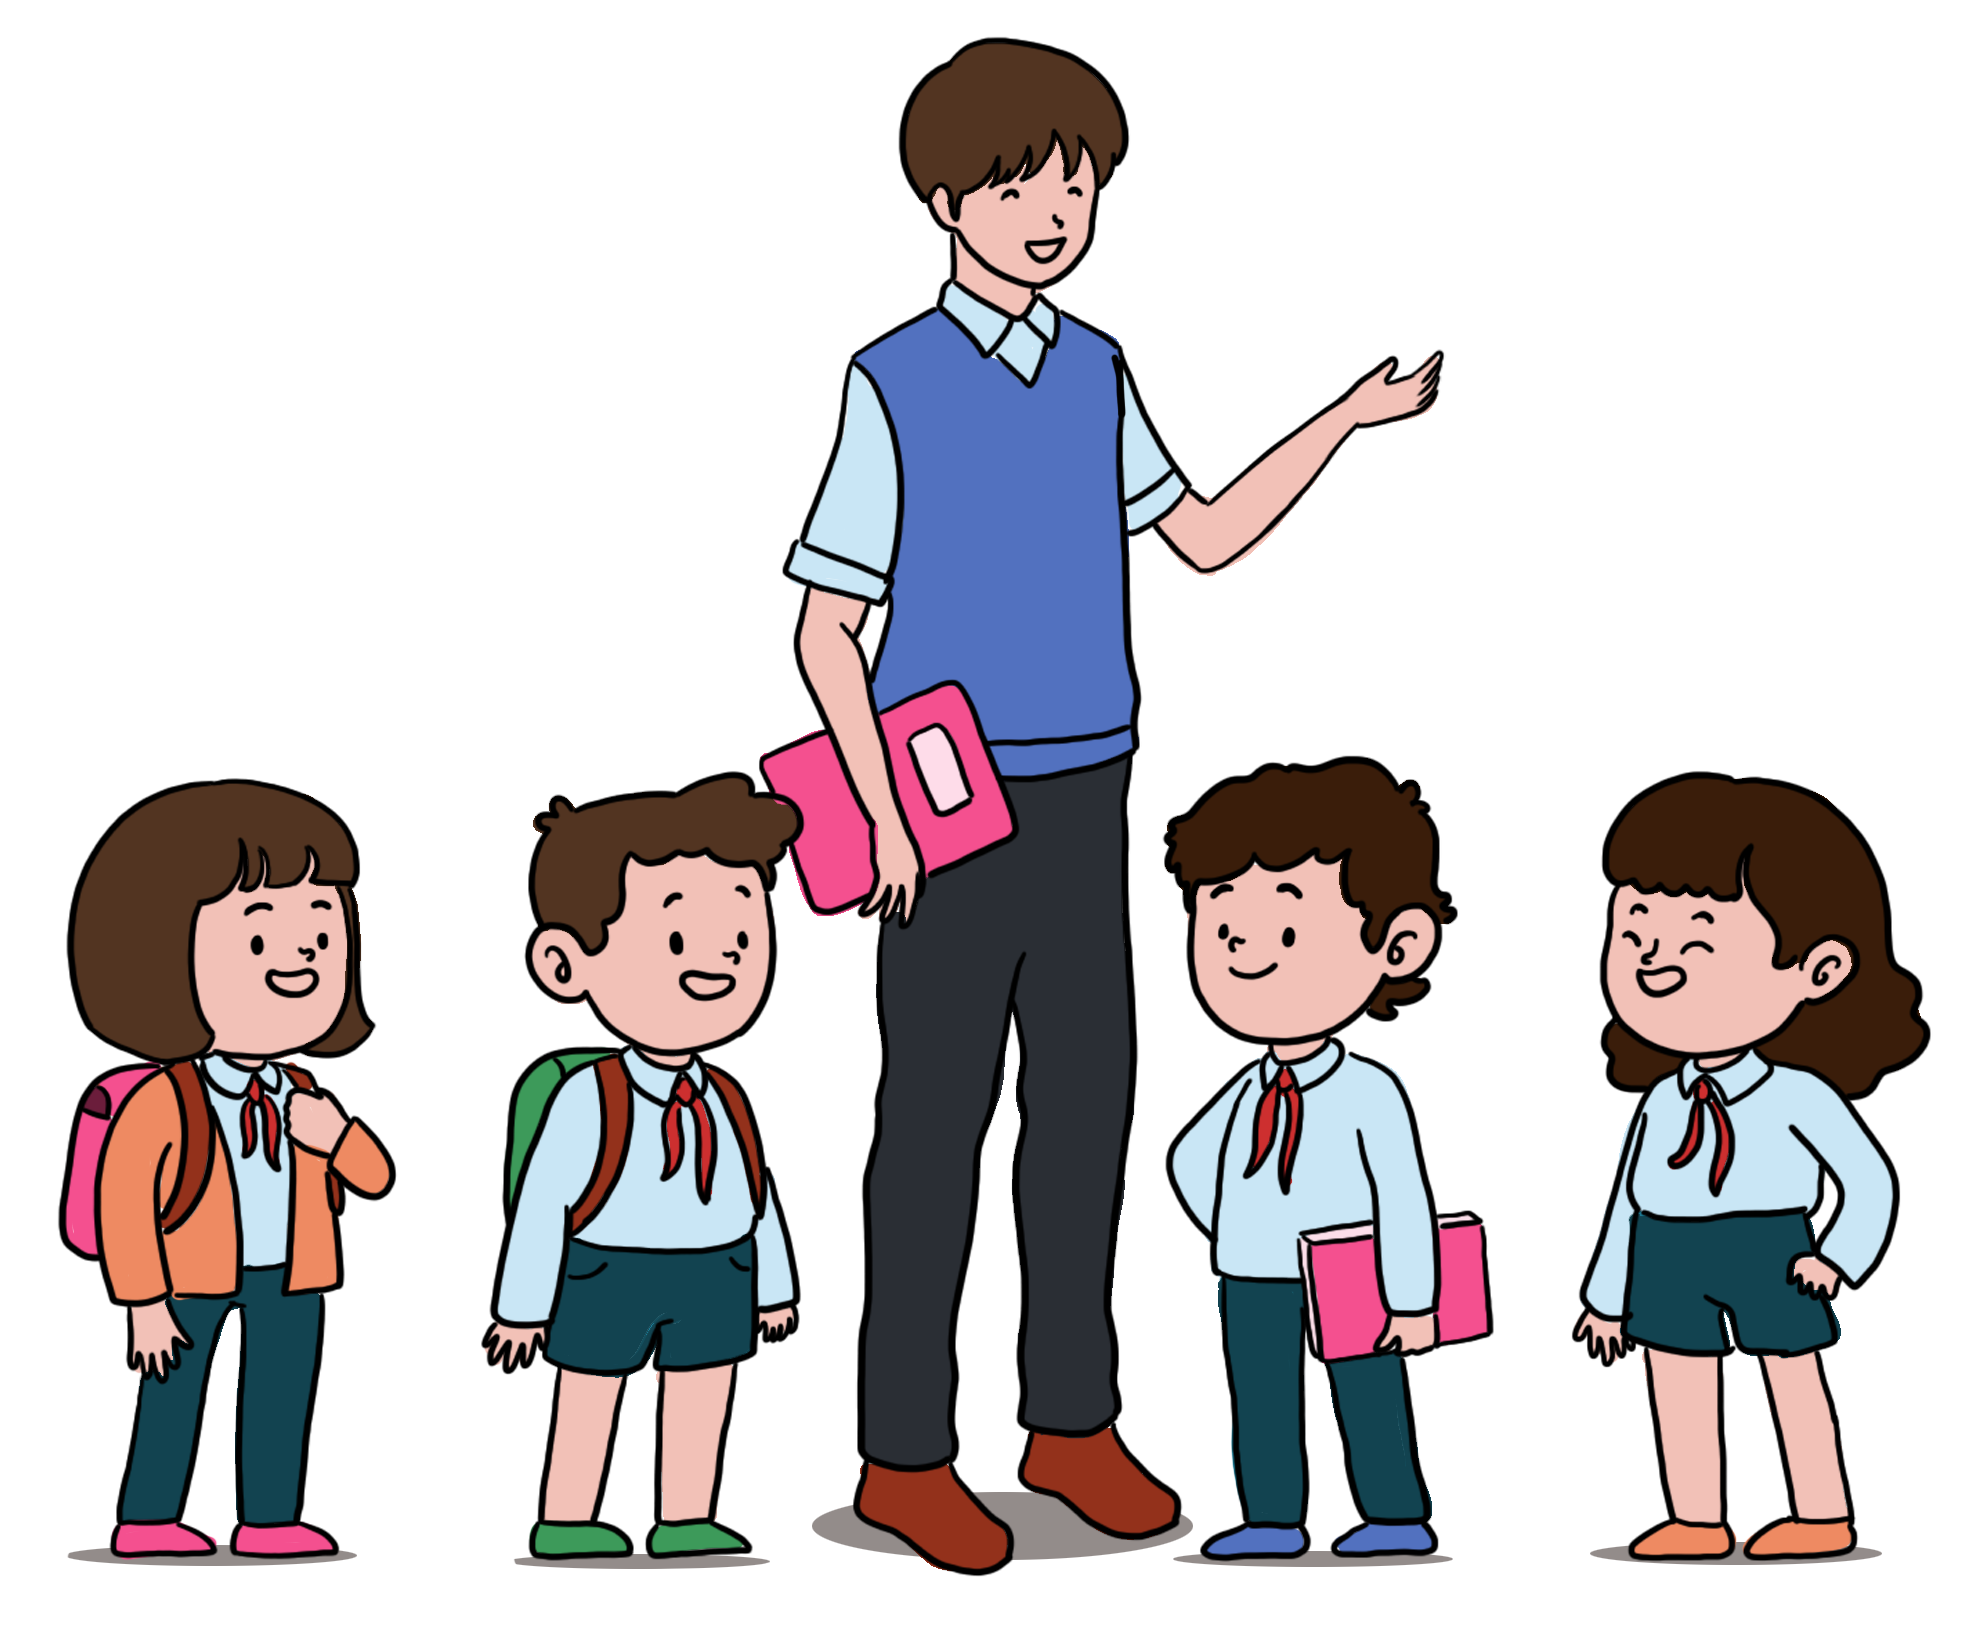
\includegraphics[width=1\linewidth]{Pi10_ToanBi_Bai5}
		\vspace*{-15pt}
	\end{figure}
	$\pmb{6.}$ $a)$  Có $50$ vị khách ngồi xung quanh một chiếc bàn tròn được xếp đều, trong số họ có $25$ phụ nữ. Em hãy chứng tỏ rằng có một vị khách ngồi cạnh hai phụ nữ.
	\vskip 0.1cm
	$b)$ Giả sử bây giờ số phụ nữ là $26$ người. Trong buổi tiệc bỗng dưng có hai vị khách làm vỡ mất hai chiếc cốc đặt trước mặt họ. Em hãy chứng tỏ rằng có thể xoay lại chiếc bàn tròn theo một cách nào đó để sao cho hai chiếc cốc vỡ lại đặt trước mặt của hai vị khách~nữ.
	\begin{figure}[H]
		\centering
		\vspace*{-10pt}
		\captionsetup{labelformat= empty, justification=centering}
		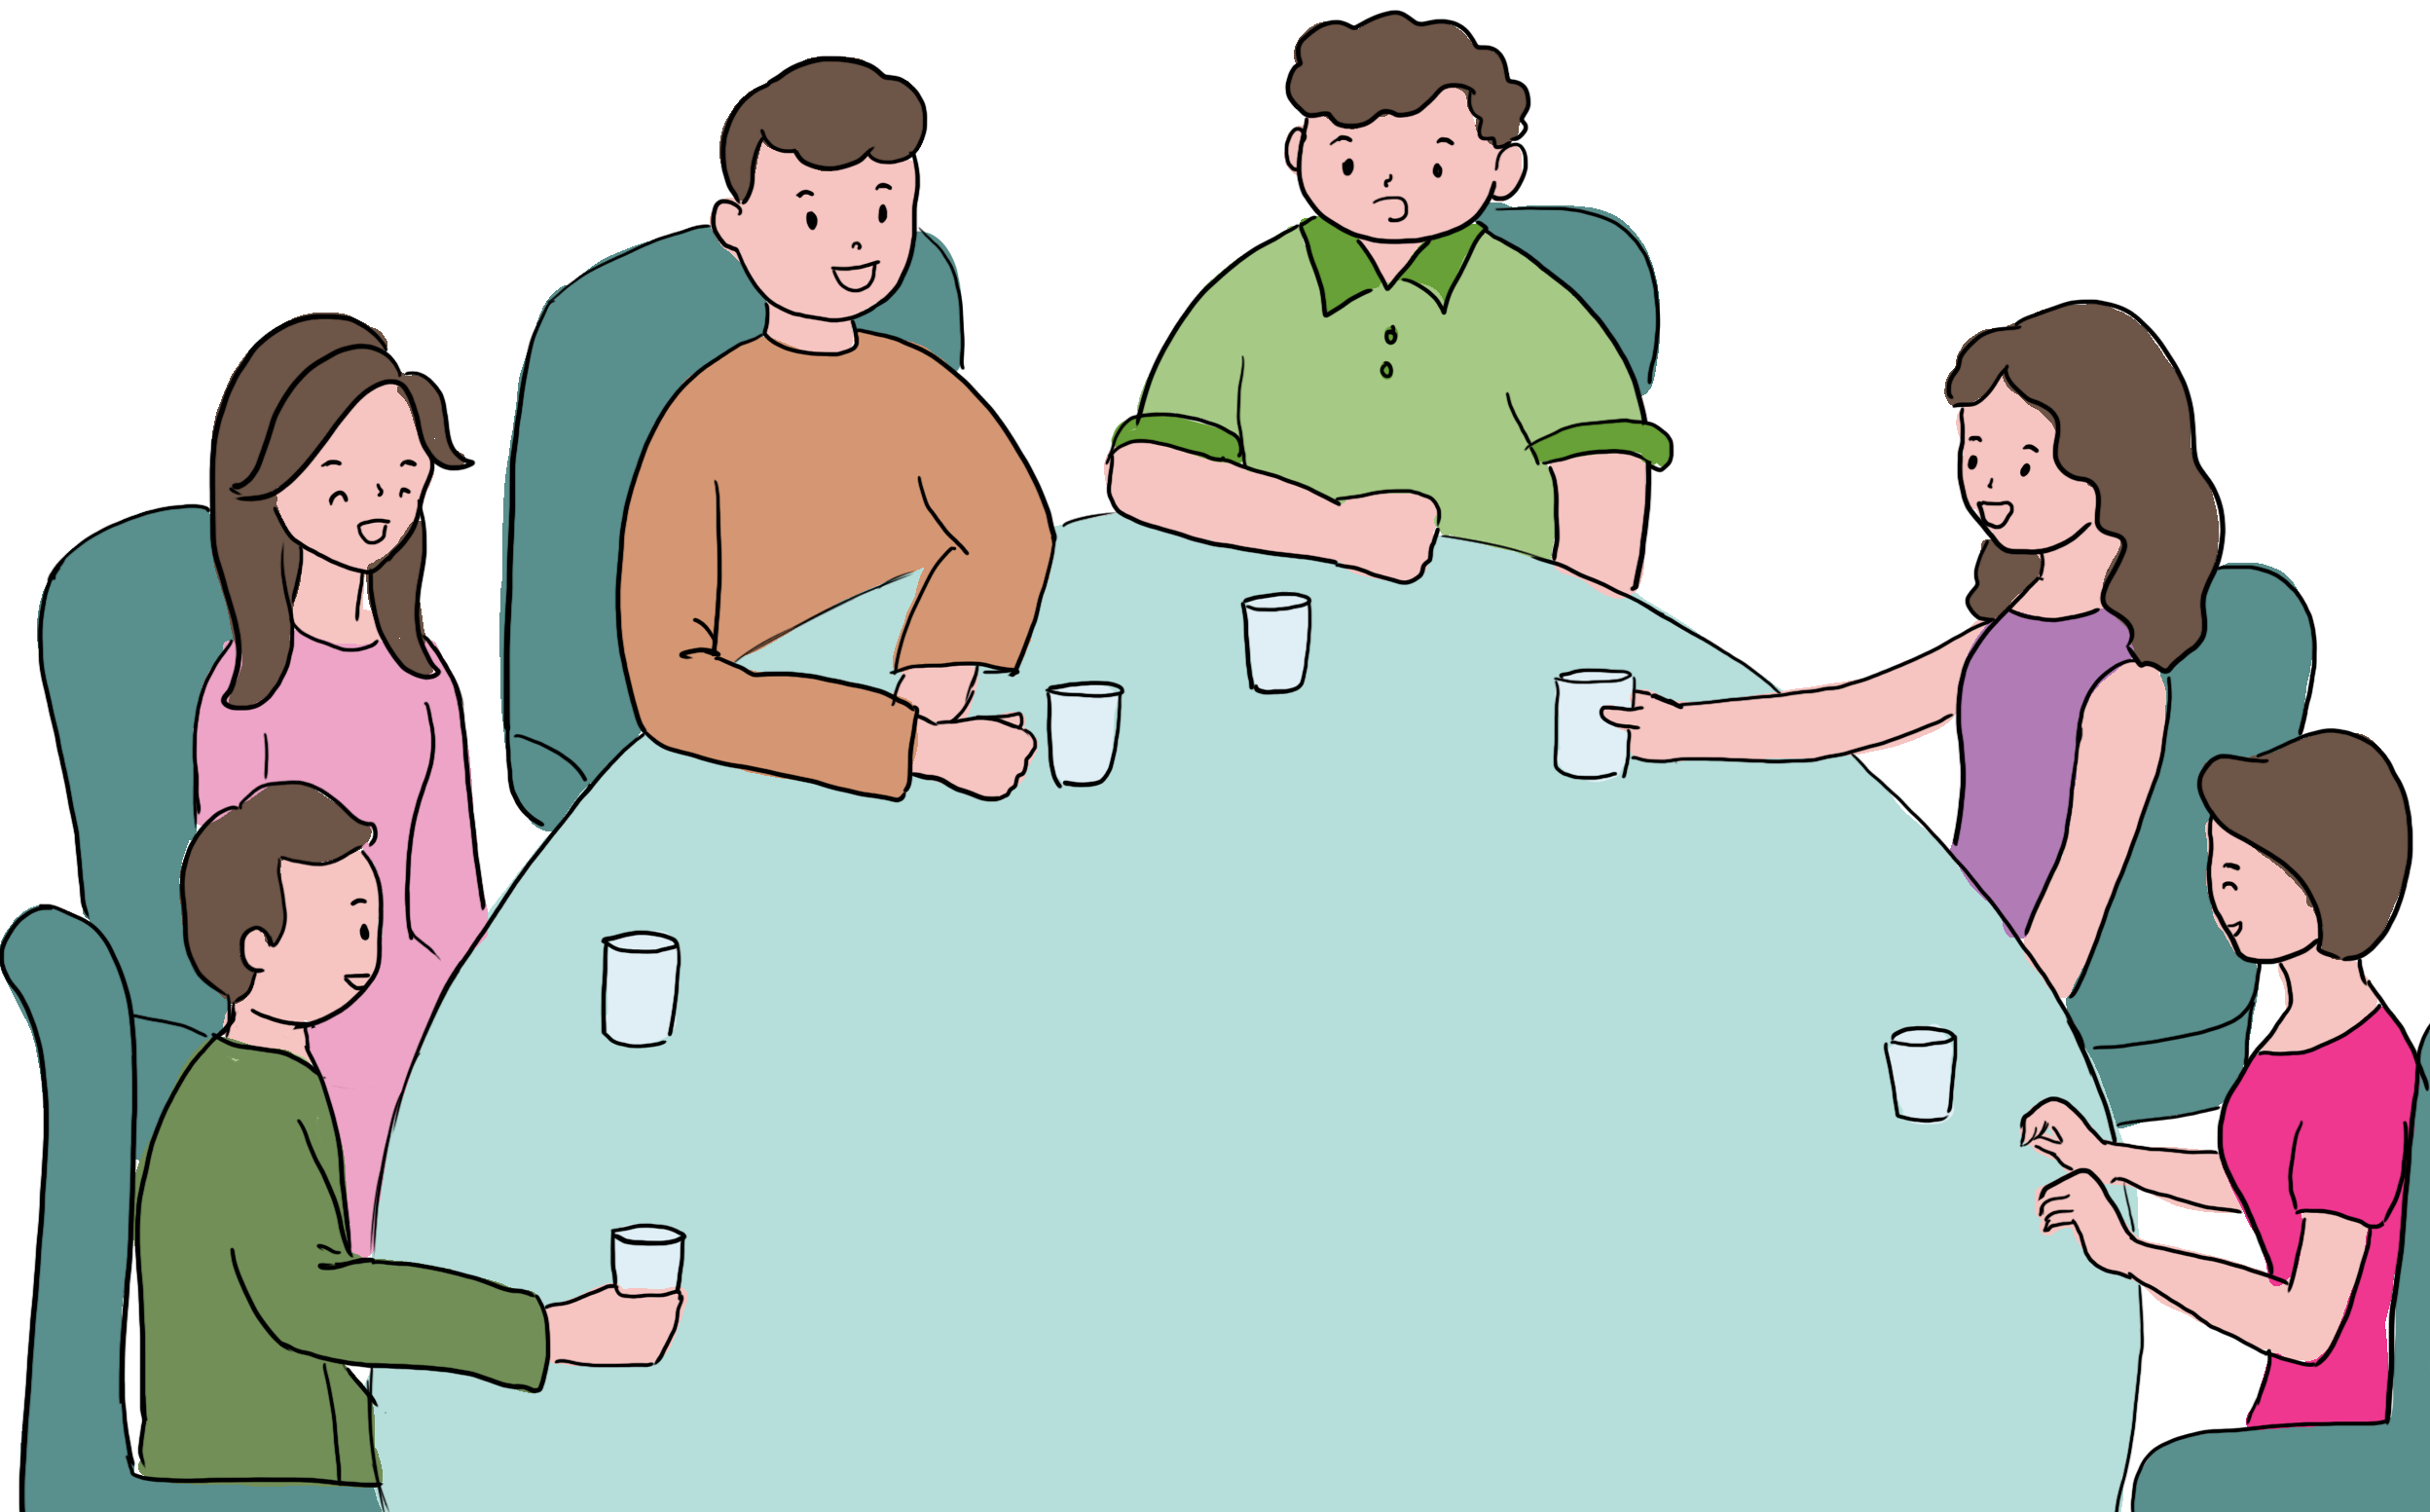
\includegraphics[width=1\linewidth]{Pi10_ToanBi_Bai6}
%		\vspace*{-5pt}
	\end{figure}
\end{multicols}
\vspace*{-10pt}
\rule{1\linewidth}{0.1pt}
\begingroup
\AddToShipoutPicture*{\put(112,374){
\includegraphics[scale=1]{../tieude2.pdf}}} 
\centering
\endgroup
\graphicspath{{../toancuabi/pic/}}
\vspace*{75pt}

\begin{multicols}{2}
	$\pmb{1.}$ Hai bạn nhỏ tham gia trò chơi Nhà đầu tư nhỏ tuổi. Bạn Vinh nói với bạn Bình: ``Nếu $3/5$ số vốn của tớ mà được thêm $7000$ đồng, thì sẽ bằng số vốn của cậu". Nghe thế, Bình liền  nhận xét: ``Vậy là vốn của cậu chỉ hơn của tớ có $3000$ đồng." Các em hãy xác định số vốn của các bạn nhỏ này nhé.
	\begin{figure}[H]
		\vspace*{-10pt}
		\centering
		\captionsetup{labelformat= empty, justification=centering}
		
\includegraphics[width= 1\linewidth]{bai1}
%		\vspace*{-5pt}
	\end{figure}
	\textit{Lời giải.} Số vốn tổng cộng của Vinh gồm $3/5$ phần vốn cộng với $2/5$ phần vốn. Nếu như Vinh thêm cả $7000$ vào số vốn của mình, thì Vinh  sẽ hơn Bình tận  $7000+3000= 10000$ (đồng). Từ đề bài ta thấy, do $3/5$ tiền vốn của Vinh cộng với $7000$ đồng đã bằng số vốn của Bình, nên $2/5$ số vốn của Vinh đúng bằng $10000$ (đồng). Vì thế số vốn của Vinh tham gia trò chơi là: $10000: (2/5)= 25000$ (đồng), và số vốn của Bình là $25000-3000=22000$ (đồng).
	\vskip 0.1cm
	$\pmb{2.}$ Có một số điểm dừng nghỉ cho người đi đường (nhiều hơn $1$) trải dọc trên một con đường dài $60$ km. Một người đi bộ dọc theo con đường với vận tốc $5$ (km$/$h) và nghỉ chân tại mỗi điểm dừng nghỉ cùng một khoảng thời gian là một số nguyên giờ đồng hồ. Một người khác đi xe đạp trên quãng đường đó với vận tốc $12$ (km$/$h) và nghỉ tại mỗi điểm dừng nghỉ với thời gian gấp đôi so với người đi bộ. Hai người cùng khởi hành và đến đích đồng thời. Hỏi có bao nhiêu điểm dừng nghỉ dọc trên đường.
	\begin{figure}[H]
		\vspace*{-8pt}
		\centering
		\captionsetup{labelformat= empty, justification=centering}
		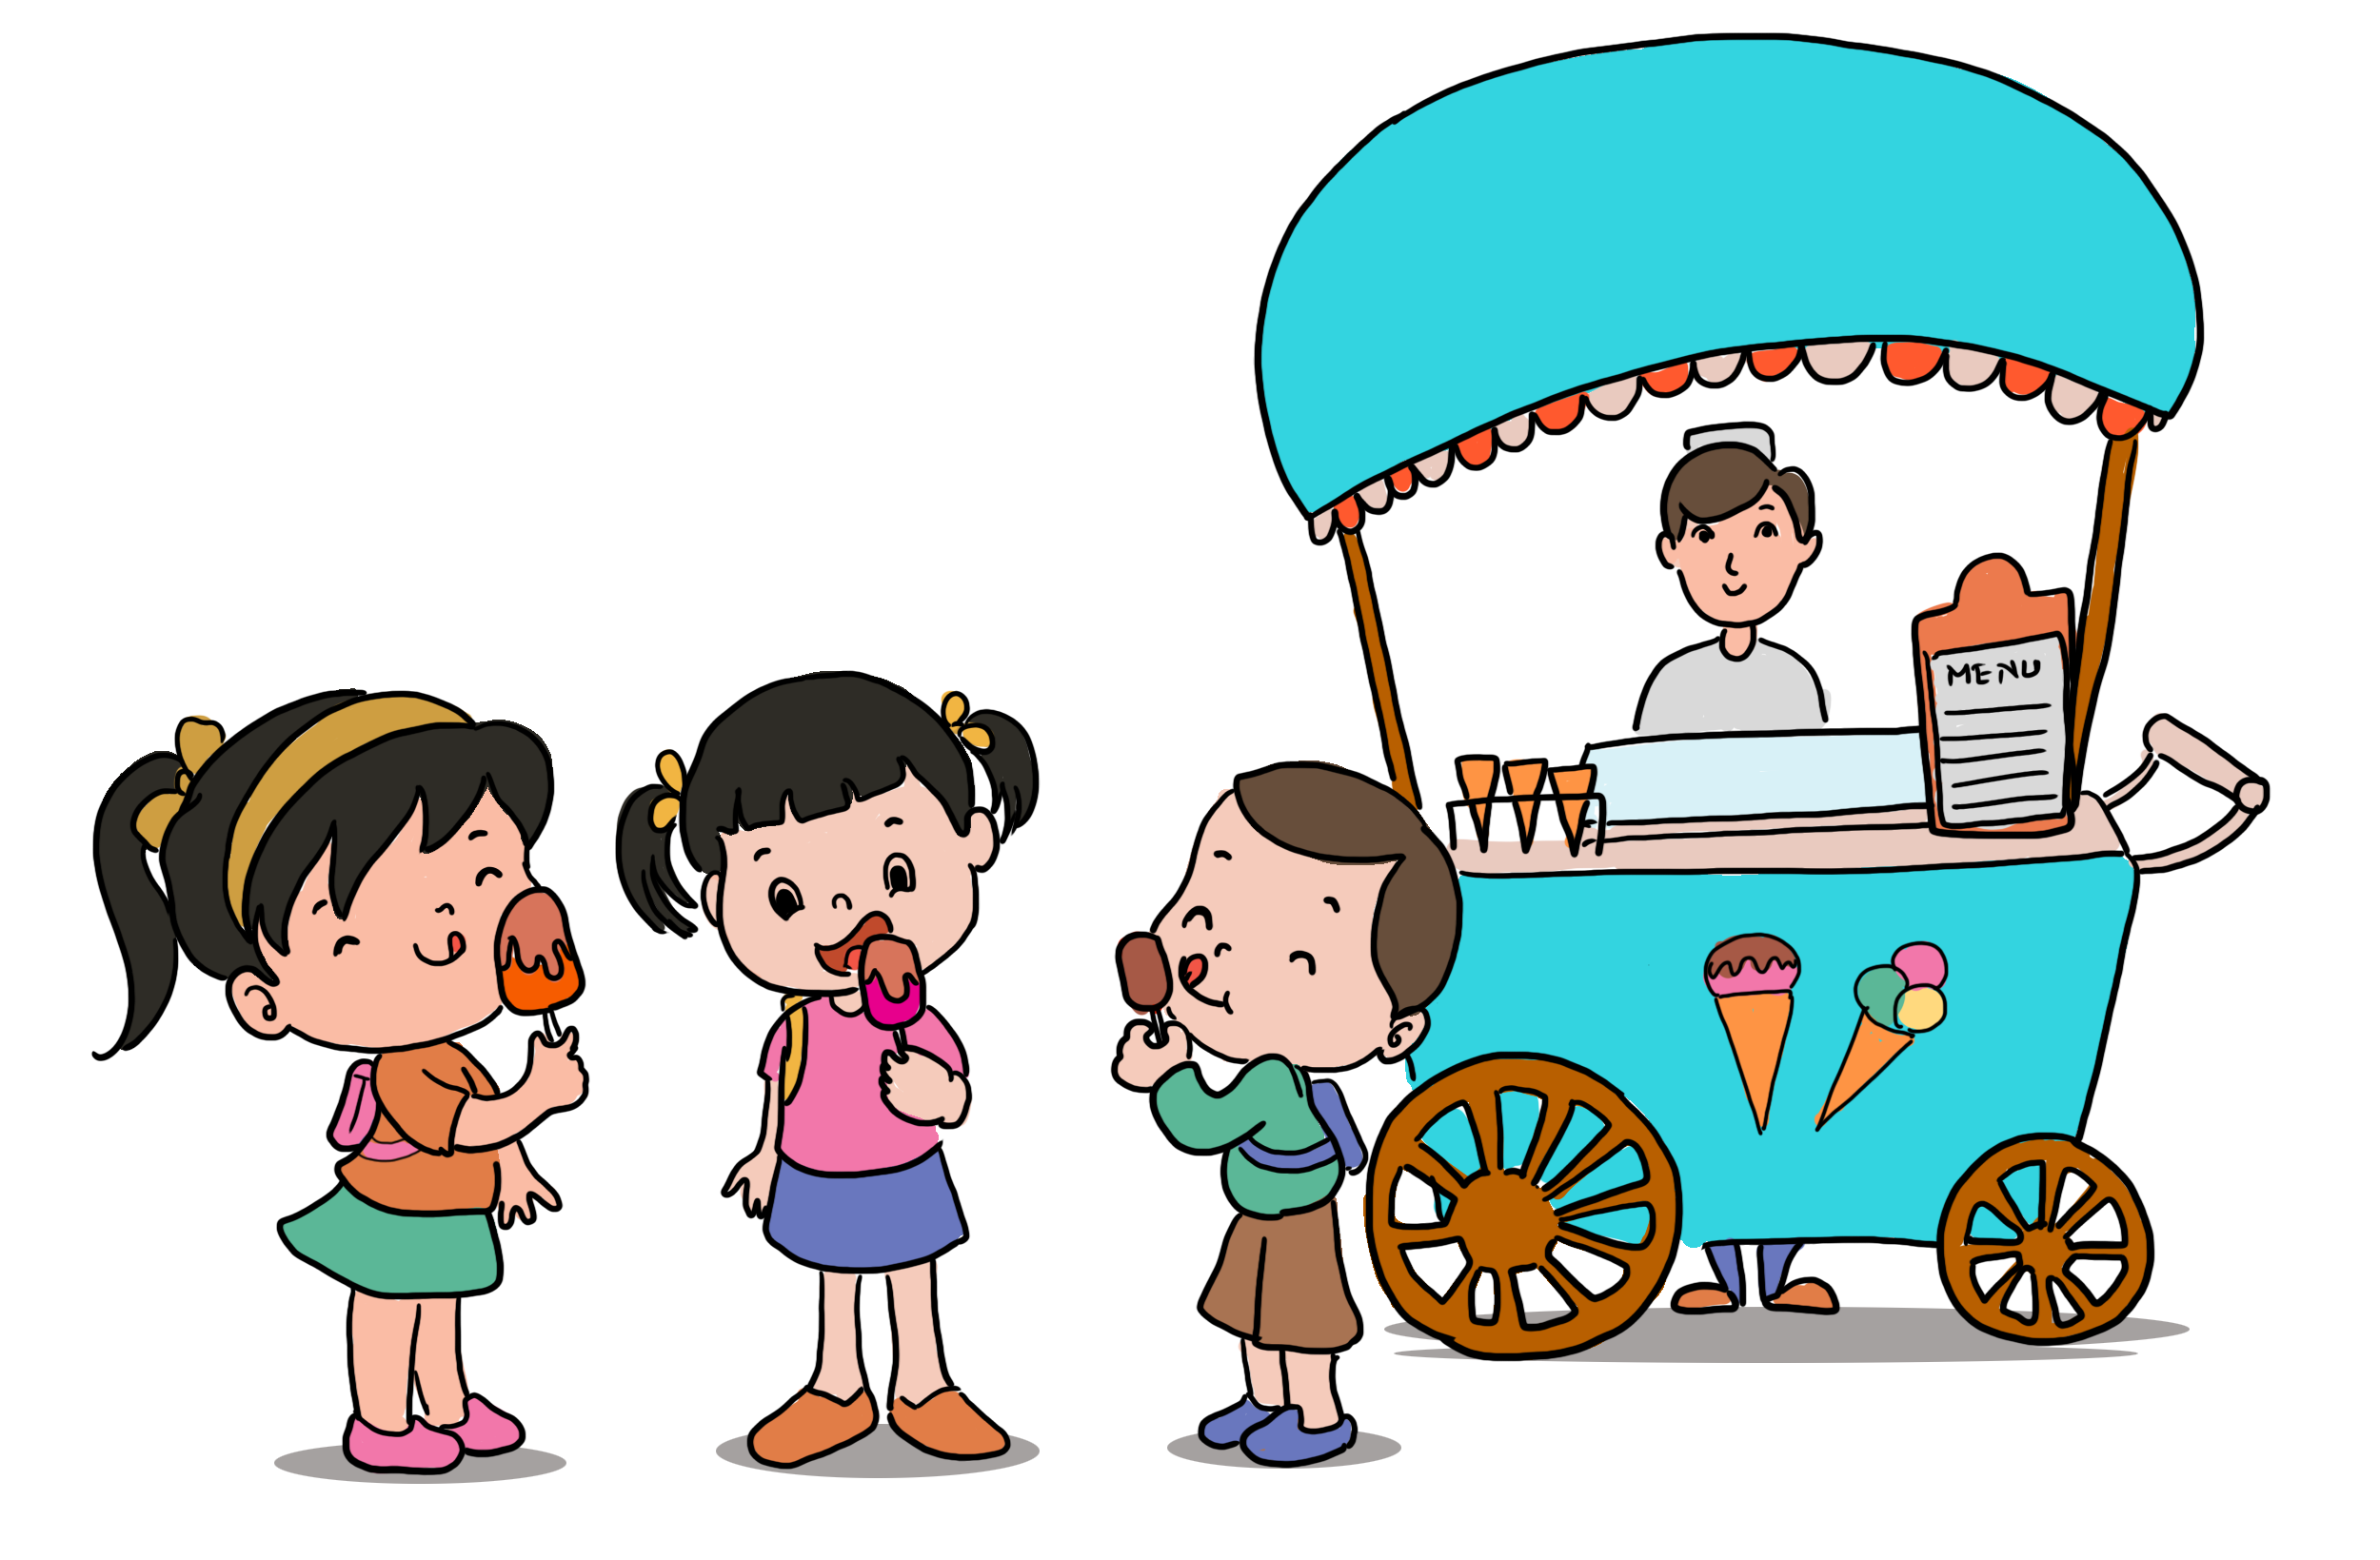
\includegraphics[width= 1\linewidth]{bai2}
		\vspace*{-15pt}
	\end{figure}
	\textit{Lời giải.} Thời gian người đi bộ đi trên đường không tính thời gian nghỉ chân là $12$ giờ. Còn người đi xe đạp mất $5$ giờ để đạp xe. Vì thế thời gian người đi xe đạp nghỉ tại các gốc cây nhiều hơn số thời gian người đi bộ nghỉ là $12-5 = 7$ (giờ). Đây cũng chính là số tiếng người đi bộ đã nghỉ tại các điểm dừng nghỉ. Vì có nhiều hơn một điểm dừng nghỉ và khoảng thời gian nghỉ tại mỗi gốc là một lượng nguyên của giờ đồng hồ, nên suy ra có $7$ điểm dừng nghỉ trên đường.
	\vskip 0.1cm
	$\pmb{3.}$ Mãng xà hay có thói bắt trộm gà của dân làng. Một lần nọ nó bị đau bụng vì ăn nhiều thịt gà sống quá nên phải tới khám bác sỹ. Bác sỹ bảo nếu Mãng xà còn ăn tới $6$ con gà sống trong một ngày thì $10$ năm nữa nó sẽ chết, còn nếu ăn tận $17$ con gà một ngày như bây giờ thì chỉ còn sống được $5$ năm nữa. Hỏi Mãng xà sẽ sống được thêm bao nhiêu năm, nếu nó chịu khó không bắt gà ăn thịt lung tung nữa. (Ta coi rằng độ dài mỗi năm là như nhau và mỗi một con gà sống làm giảm tuổi thọ một số thời gian như nhau).
	\begin{figure}[H]
		\vspace*{-8pt}
		\centering
		\captionsetup{labelformat= empty, justification=centering}
		
\includegraphics[width= 0.9\linewidth]{bai3}
		\vspace*{-5pt}
	\end{figure}
	\vskip 0.1cm
	Ta gọi số ngày trong năm là $n$. Khi đó $6\cdot10n= 60n$ là số gà ăn vào sẽ làm giảm tuổi thọ của Mãng xà để nó chỉ sống thêm được $10$ năm nữa. Còn $17\cdot5n = 85n$ là số gà ăn vào sẽ làm giảm tuổi thọ của Mãng xà để nó chỉ sống thêm được $5$ năm. Như vậy $85n-60n = 25n$ con gà sẽ làm giảm tuổi thọ của Mãng xà mất $5$ năm. Như vậy, nếu Mãng xà thôi không bắt gà sống ăn thịt thì nó sẽ sống thêm được $10$ năm cộng với số năm mà $60n$ con gà có thể đã tước đoạt đi tuổi thọ của nó, có nghĩa là $(60:25)\cdot5 = 12$ (năm).
	\vskip 0.1cm	
	Vậy nếu không bắt gà  của dân làng nữa, Mãng xà có thể sống thêm được $10+ 12 = 22$ (năm).
	\vskip 0.1cm
	$\pmb{4.}$ Có thể đặt các số tự nhiên từ $1$ tới $15$ vào một bảng vuông hình chữ nhật $3\times 5$ sao cho tổng các số trong mỗi hàng là như nhau và tổng các số trong mỗi cột cũng như nhau được hay không?
	\vskip 0.1cm
	Có thể. ta đưa ra một ví dụ như sau
	\begin{figure}[H]
		\centering
		\vspace*{-5pt}
		\captionsetup{labelformat= empty, justification=centering}
		\begin{tikzpicture}[toancuabi,scale=0.85]
			\draw (0,0) grid (5,3);
			\node at (0.5,0.5) {$15$};
			\node at (1.5,0.5) {$10$};
			\node at (2.5,0.5) {$6$};
			\node at (3.5,0.5) {$2$};
			\node at (4.5,0.5) {$7$};
			\node at (0.5,1.5) {$8$};
			\node at (1.5,1.5) {$3$};
			\node at (2.5,1.5) {$4$};
			\node at (3.5,1.5) {$13$};
			\node at (4.5,1.5) {$12$};
			\node at (0.5,2.5) {$1$};
			\node at (1.5,2.5) {$11$};
			\node at (2.5,2.5) {$14$};
			\node at (3.5,2.5) {$9$};
			\node at (4.5,2.5) {$5$};
		\end{tikzpicture}
		\vspace*{-5pt}
	\end{figure}
	Sau đây là một số gợi ý:
	\vskip 0.1cm
	-- Trước tiên ta biết tổng của $15$ số bằng $(15\times16):2=120$. Do đó tổng của mỗi cột (nếu xếp được) là $24$, còn tổng mỗi hàng bằng $40$. Theo suy nghĩ thông thường ta chọn $3$ số cách đều $1$, $8$, $15$ cho cột đầu tiên.
	\vskip 0.1cm
	-- Xem xét $5$ số lớn nhất còn lại ta thấy $10$ và $11$ phải cùng một cột và cùng với số $3$. Ta xếp ba số $3$, $10$, $11$ vào cột hai (tạm thời chưa xếp vào các dòng). 
	\vskip 0.1cm
	-- Tiếp theo, trong các ô ở $3$ cột còn lại (cột thứ $3$ tới cột thứ $5$) ta sẽ xếp số lớn nhất $(14)$ cùng hàng với $1$ và số bé nhất $(2)$ cùng hàng với $15$ (cũng theo nguyên tắc xếp dãn đều). Thấy ngay $14$ và $2$ không thể ở cùng một cột, vì nếu như vậy, ô còn lại phải ghi số $8$ là số ta đã xếp ở cột $1$. Quay lại cột $2$, bằng cách xét từng trường hợp ta chỉ có thể  xếp số $3$ vào ô $G$ (Hình $1$).
	\begin{table}[H]
		\vspace*{-5pt}
		\centering
		\captionsetup{labelformat= empty, justification=centering}
		\renewcommand{\arraystretch}{1.23}
		\begin{tabular}{|c|c|c|c|c|}
			\hline
			$1$ & & $14$& & \\
			$A$&$B$&$C$&$D$& $E$\\
			\hline
			 $8$&$3$&&&\\
			 $F$&$G$&$H$&$I$&$J$\\
			 \hline
			 $15$&&&$2$&\\
			 $K$&$L$&$M$&$N$&$P$\\
			 \hline
		\end{tabular}
		\caption{\small\textit{\color{toancuabi}Hình $1$.}}
		\vspace*{-10pt}
	\end{table}
	-- Tiếp theo do tổng các ô $H$, $I$ và $J$ sẽ bằng $40-(8+3)= 29$ các ô này phải có cả hai số ``lớn" còn lại là $12$ và $13$ và ô còn lại trong $3$ ô này phải là số $4$. Xét $3$ trường hợp cho ô $I$ ta thấy chỉ có thể điền $13$ vào ô $I$.  Khi đó ta điền tiếp được các ô $H$, $J$, $D$, $M$ (Hình $2$)
	\begin{table}[H]
		\vspace*{-5pt}
		\centering
		\captionsetup{labelformat= empty, justification=centering}
		\renewcommand{\arraystretch}{1.23}
		\begin{tabular}{|c|c|c|c|c|}
			\hline
			$1$ & & $14$&$9$ & \\
			$A$&$B$&$C$&$D$& $E$\\
			\hline
			$8$&$3$&$4$&$13$&$12$\\
			$F$&$G$&$H$&$I$&$J$\\
			\hline
			$15$&&$6$&$2$&\\
			$K$&$L$&$M$&$N$&$P$\\
			\hline
		\end{tabular}
		\caption{\small\textit{\color{toancuabi}Hình $2$.}}
		\vspace*{-10pt}
	\end{table}
	-- Chỉ có thể điền $11$ vào ô $B$ và cuối cùng thu được toàn bộ bảng ở Hình $3$.
	\begin{table}[H]
		\vspace*{-5pt}
		\centering
		\captionsetup{labelformat= empty, justification=centering}
		\renewcommand{\arraystretch}{1.23}
		\begin{tabular}{|c|c|c|c|c|}
			\hline
			$1$ &$11$&$14$&$9$&$5$ \\
			$A$&$B$&$C$&$D$& $E$\\
			\hline
			$8$&$3$&$4$&$13$&$12$\\
			$F$&$G$&$H$&$I$&$J$\\
			\hline
			$15$&$10$&$6$&$2$&$7$\\
			$K$&$L$&$M$&$N$&$P$\\
			\hline
		\end{tabular}
		\caption{\small\textit{\color{toancuabi}Hình $3$.}}
		\vspace*{-10pt}
	\end{table}
	Các em cũng có thể đổi chỗ các cột, hoặc các hàng để có một cách điền khác.
	\vskip 0.1cm
	$\pmb{5.}$ Hai bạn cùng chơi một trò tô màu sau đây: các bạn lần lượt tô bằng màu đỏ các ô của một bảng ô vuông ca--rô $4\times 4$. Ở mỗi một bước, các bạn phải tô một ô trắng bằng màu đỏ, sao cho không có hình vuông $2\times 2$ nào bị tô đỏ hết. Bạn nào không đi được bước tiếp theo sẽ bị thua. Hỏi bạn nào sẽ luôn có cách chơi để thắng đối phương: bạn tô đầu tiên hay là người chơi cùng với bạn đó? 
	\begin{figure}[H]
		\vspace*{-5pt}
		\centering
		\captionsetup{labelformat= empty, justification=centering}
		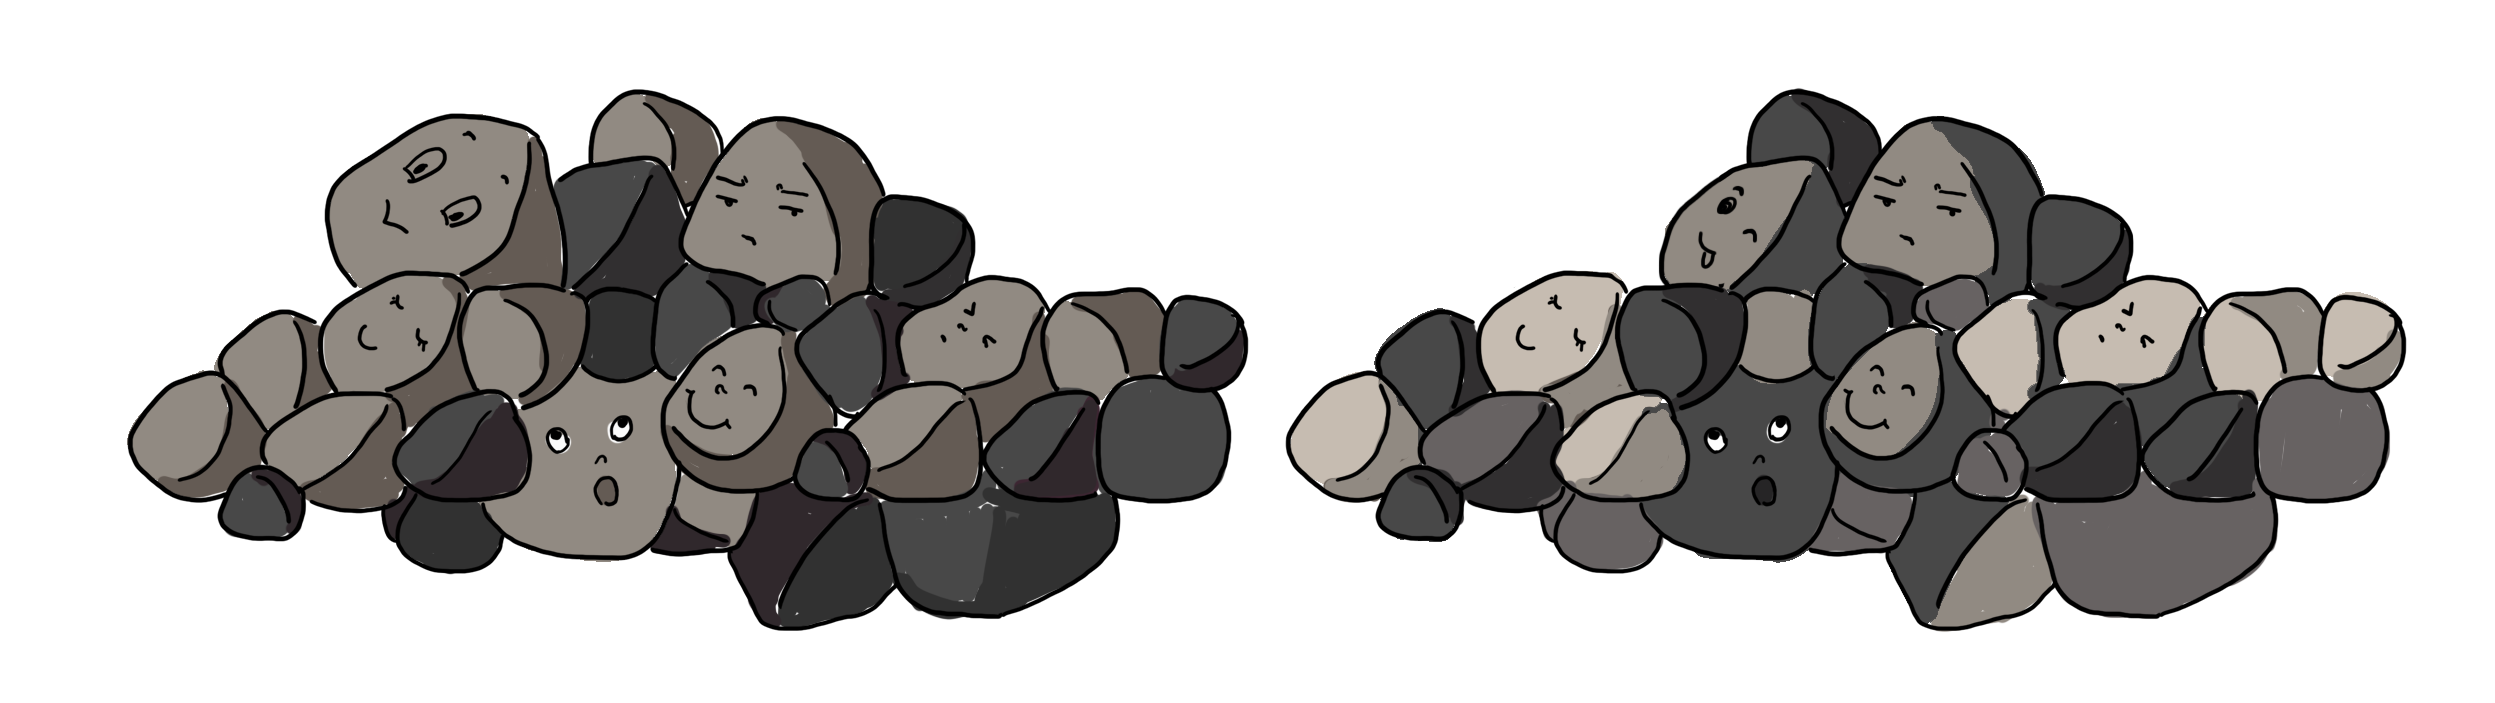
\includegraphics[width= 1\linewidth]{bai5}
		\vspace*{-15pt}
	\end{figure}
	\textit{Lời giải.} Ta đánh số $16$ ô của bàn cờ caro như sau
	\begin{figure}[H]
		\centering
		\vspace*{-5pt}
		\captionsetup{labelformat= empty, justification=centering}
		\begin{tikzpicture}[toancuabi,scale=0.85]
			\draw (0,0) grid (4,4);
			\node at (0.5,0.5) {$5$};
			\node at (1.5,0.5) {$6$};
			\node at (2.5,0.5) {$7$};
			\node at (3.5,0.5) {$8$};
			\node at (0.5,1.5) {$1$};
			\node at (1.5,1.5) {$2$};
			\node at (2.5,1.5) {$3$};
			\node at (3.5,1.5) {$4$};
			\node at (0.5,2.5) {$5$};
			\node at (1.5,2.5) {$6$};
			\node at (2.5,2.5) {$7$};
			\node at (3.5,2.5) {$8$};
			\node at (0.5,3.5) {$1$};
			\node at (1.5,3.5) {$2$};
			\node at (2.5,3.5) {$3$};
			\node at (3.5,3.5) {$4$};
		\end{tikzpicture}
		\vspace*{-5pt}
	\end{figure}
	Người chơi thứ hai (đối thủ của người đi trước) sẽ luôn có thể thắng bằng chiến thuật sau đây: hễ người thứ nhất tô màu vào ô nào trong số $16$ ô trong bảng, người chơi thứ hai sẽ tô vào ô có cùng số với ô vừa được người thứ nhất đã tô. Do không có hình vuông $2\times2$ nào trong bàn cờ có $2$ số giống nhau nên người thứ hai không bao giờ bị đẩy vào tình huống thua vì không đi được bước tiếp theo.
	\vskip 0.1cm
	$\pmb{6.}$ Có $31$ người cùng ngồi xung quanh một chiếc bàn tròn. Một số người trong họ là các Hiệp sỹ -- đó là những người luôn nói thật, còn những người còn lại là Lừa dối -- họ luôn nói sai, hơn nữa số người Lừa dối ít nhất là $1$. Người ta hỏi mỗi người trong số họ ``có bao nhiêu người Lừa dối ngồi cạnh anh?" (tức là người ngồi cạnh bên tay trái và bên tay phải). Tất cả mọi người cùng đưa ra câu trả lời như nhau. Hỏi số Hiệp sỹ lớn nhất có thể ngồi xung quanh bàn là bao nhiêu?
	\begin{figure}[H]
		\vspace*{-5pt}
		\centering
		\captionsetup{labelformat= empty, justification=centering}
		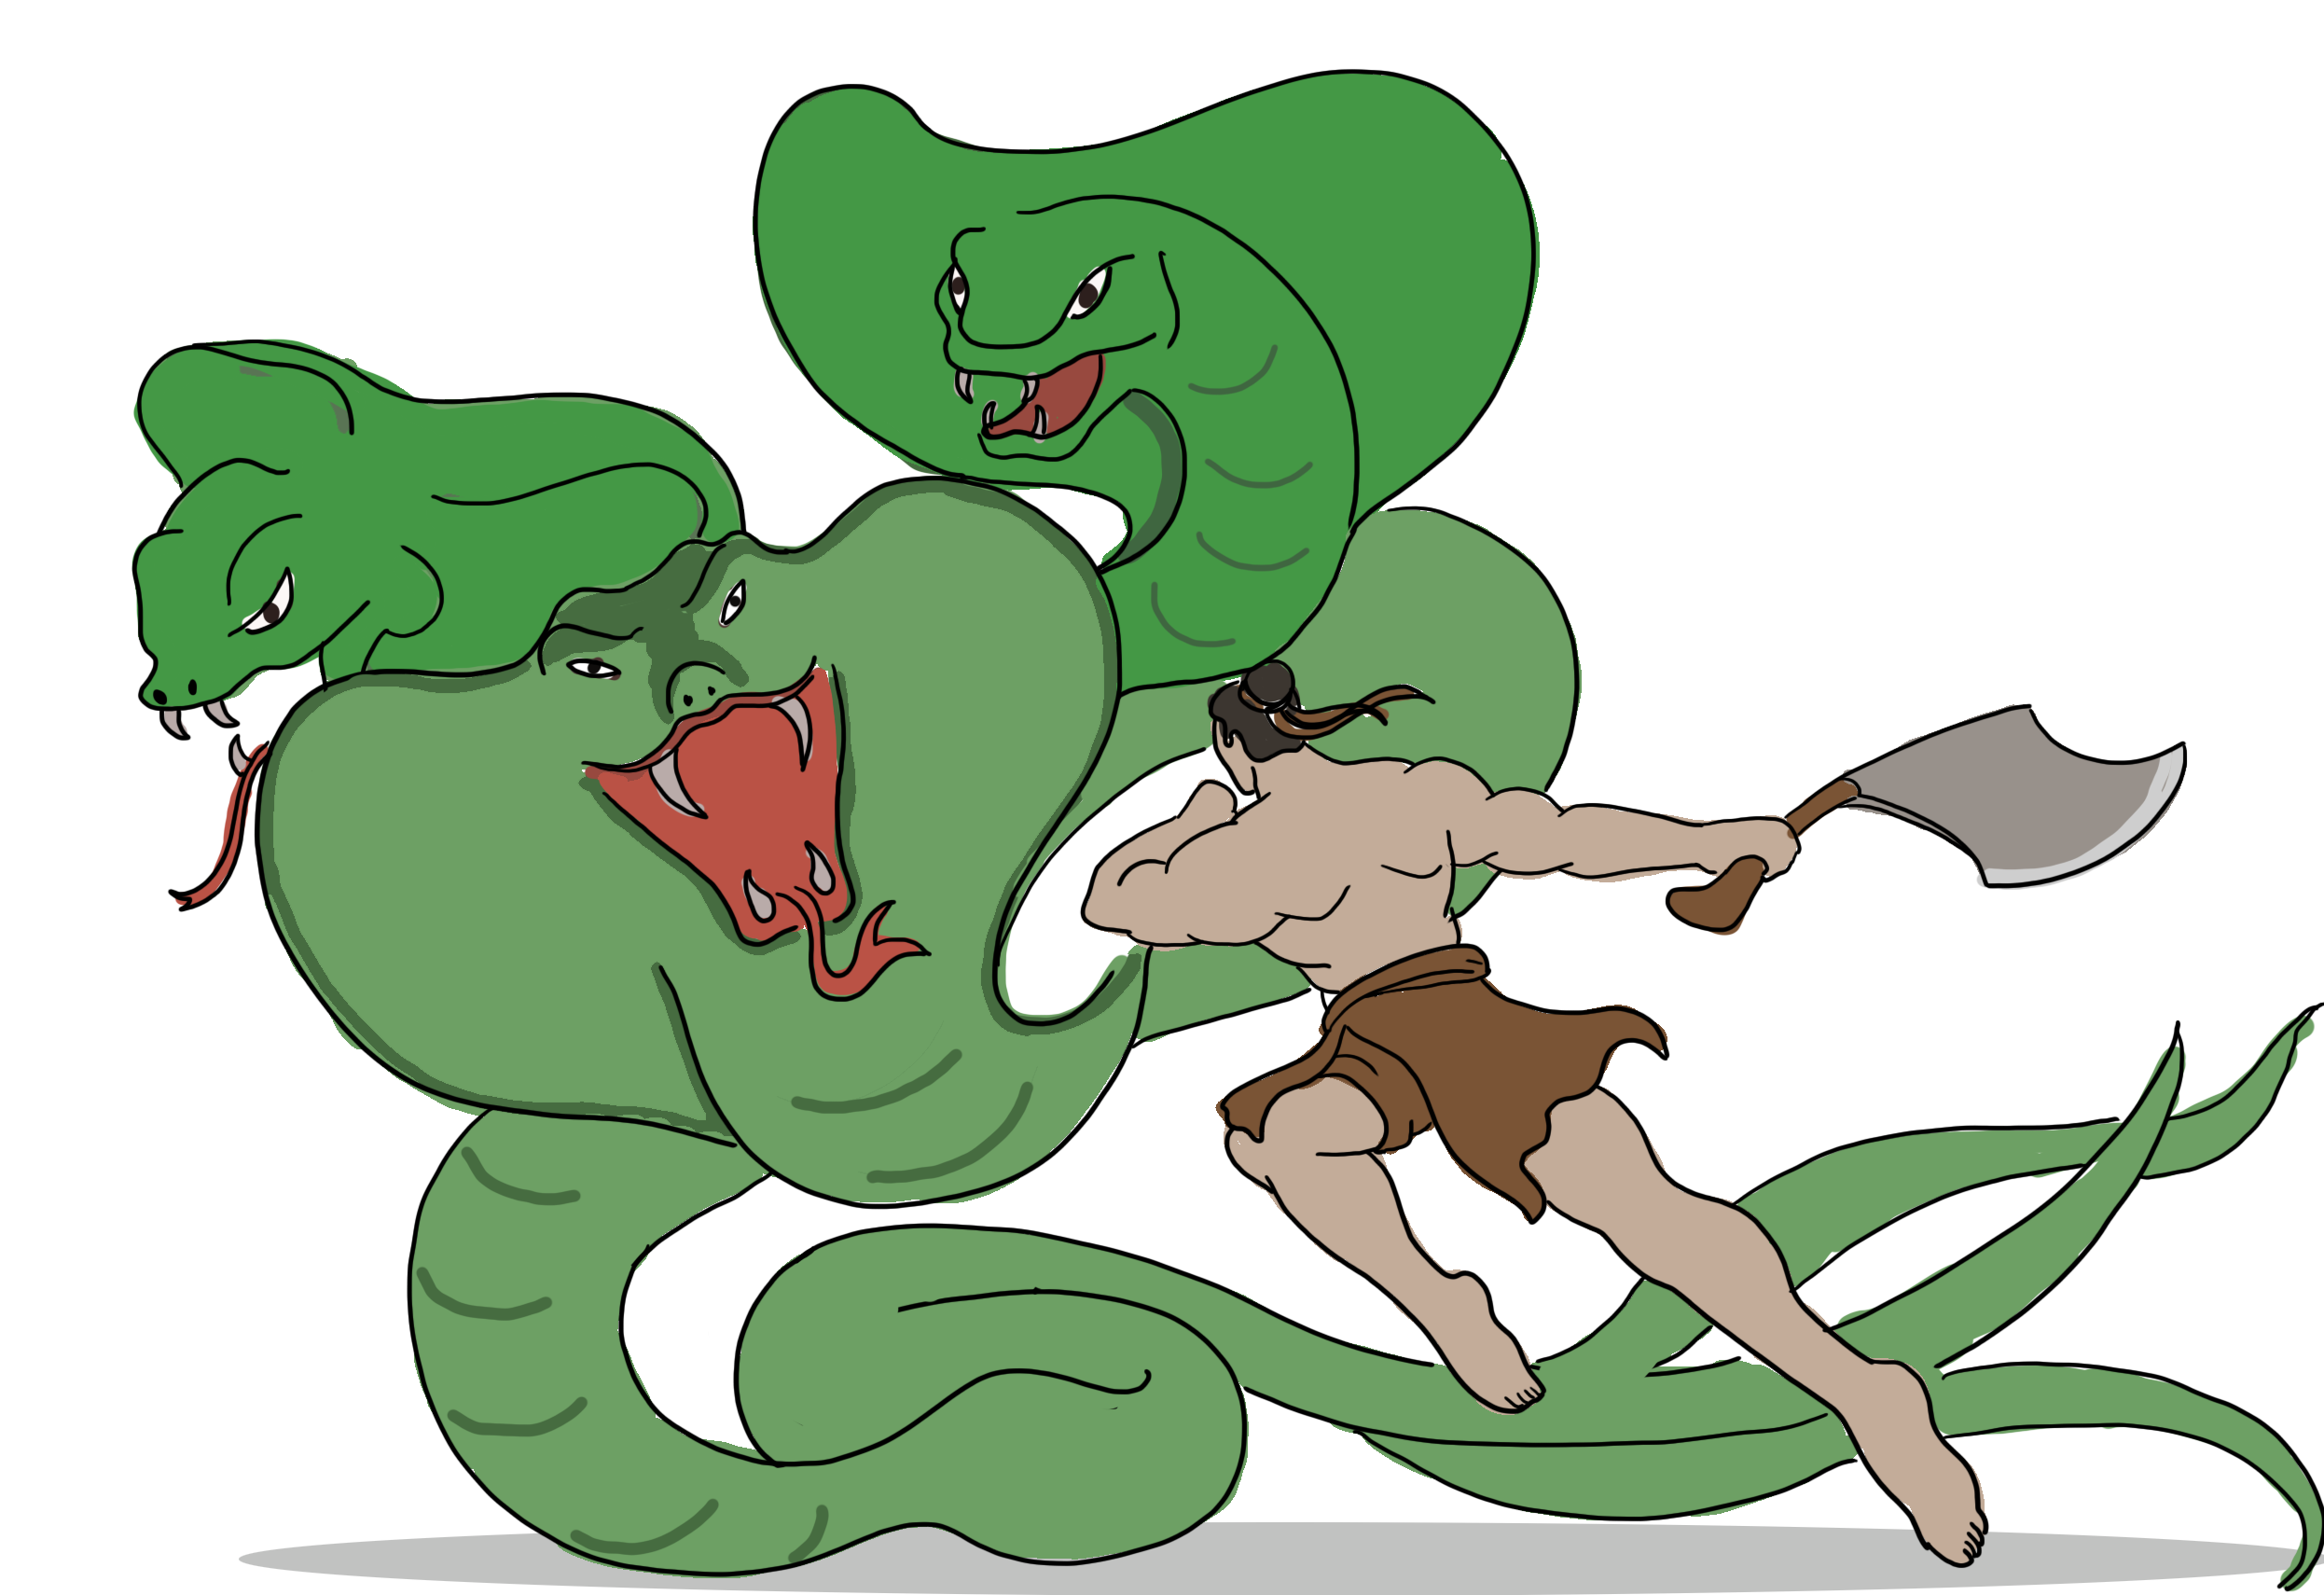
\includegraphics[width= 1\linewidth]{bai6}
		\vspace*{-10pt}
	\end{figure}
	\textit{Lời giải.} Giả sử xung quanh bàn có ít nhất $16$ Hiệp sỹ. Khi đó phải có ít  nhất $2$ Hiệp sỹ ngồi cạnh nhau. Hơn nữa vì số người Lừa dối có ít nhất là $1$, nên phải có $2$ Hiệp sỹ ngồi cạnh nhau, và một trong số họ có một người Lừa dối ngồi cạnh. Như vậy, có một Hiệp sỹ đưa ra câu trả lời là ``$1$", và tất cả cũng đã đều trả lời là ``$1$".
	\vskip 0.1cm 
	Vì thế các Hiệp sỹ phải ngồi theo từng cặp, mỗi một cặp Hiệp sỹ được bao quanh bởi các người Lừa dối. Hơn nữa, mỗi một người Lừa dối phải được bao quanh bởi $2$ Hiệp sỹ (vì nếu có một người Lừa dối có $2$ người ngồi cạnh là Hiệp sỹ và Lừa dối khác, thì hóa ra anh ta lại nói thật, điều này là không thể. Do đó chỉ có thể có cách xếp như sau
	\begin{align*}
		\ldots\text{\scriptsize{HHLHHLHHL}}\ldots
	\end{align*}
	(H -- Hiệp sỹ, L -- Lừa dối). Nhưng khi đó thì tổng số người phải là bội số của $3$. Đây là điều mâu thuẫn. Do vậy số Hiệp sỹ không quá $15$.
	\vskip 0.1cm
	Ta sẽ chỉ ra ví dụ khi có đúng $15$ Hiệp sỹ ngồi quanh bàn như sau
	\begin{align*}
		\text{\scriptsize{LHLHLHLHLHLHLHLHLHLHLHLHLHLHLLH}}
	\end{align*}
	(người đầu và người cuối trong dãy trên ngồi cạnh nhau). Khi đó mỗi người ở quanh bàn đều trả lời ``$2$".
\end{multicols}
\newpage
\begingroup
\thispagestyle{toancuabinone}
\blfootnote{$^1$\color{toancuabi}Trường THCS Archimedes, Hà Nội.}
\AddToShipoutPicture*{\put(60,733){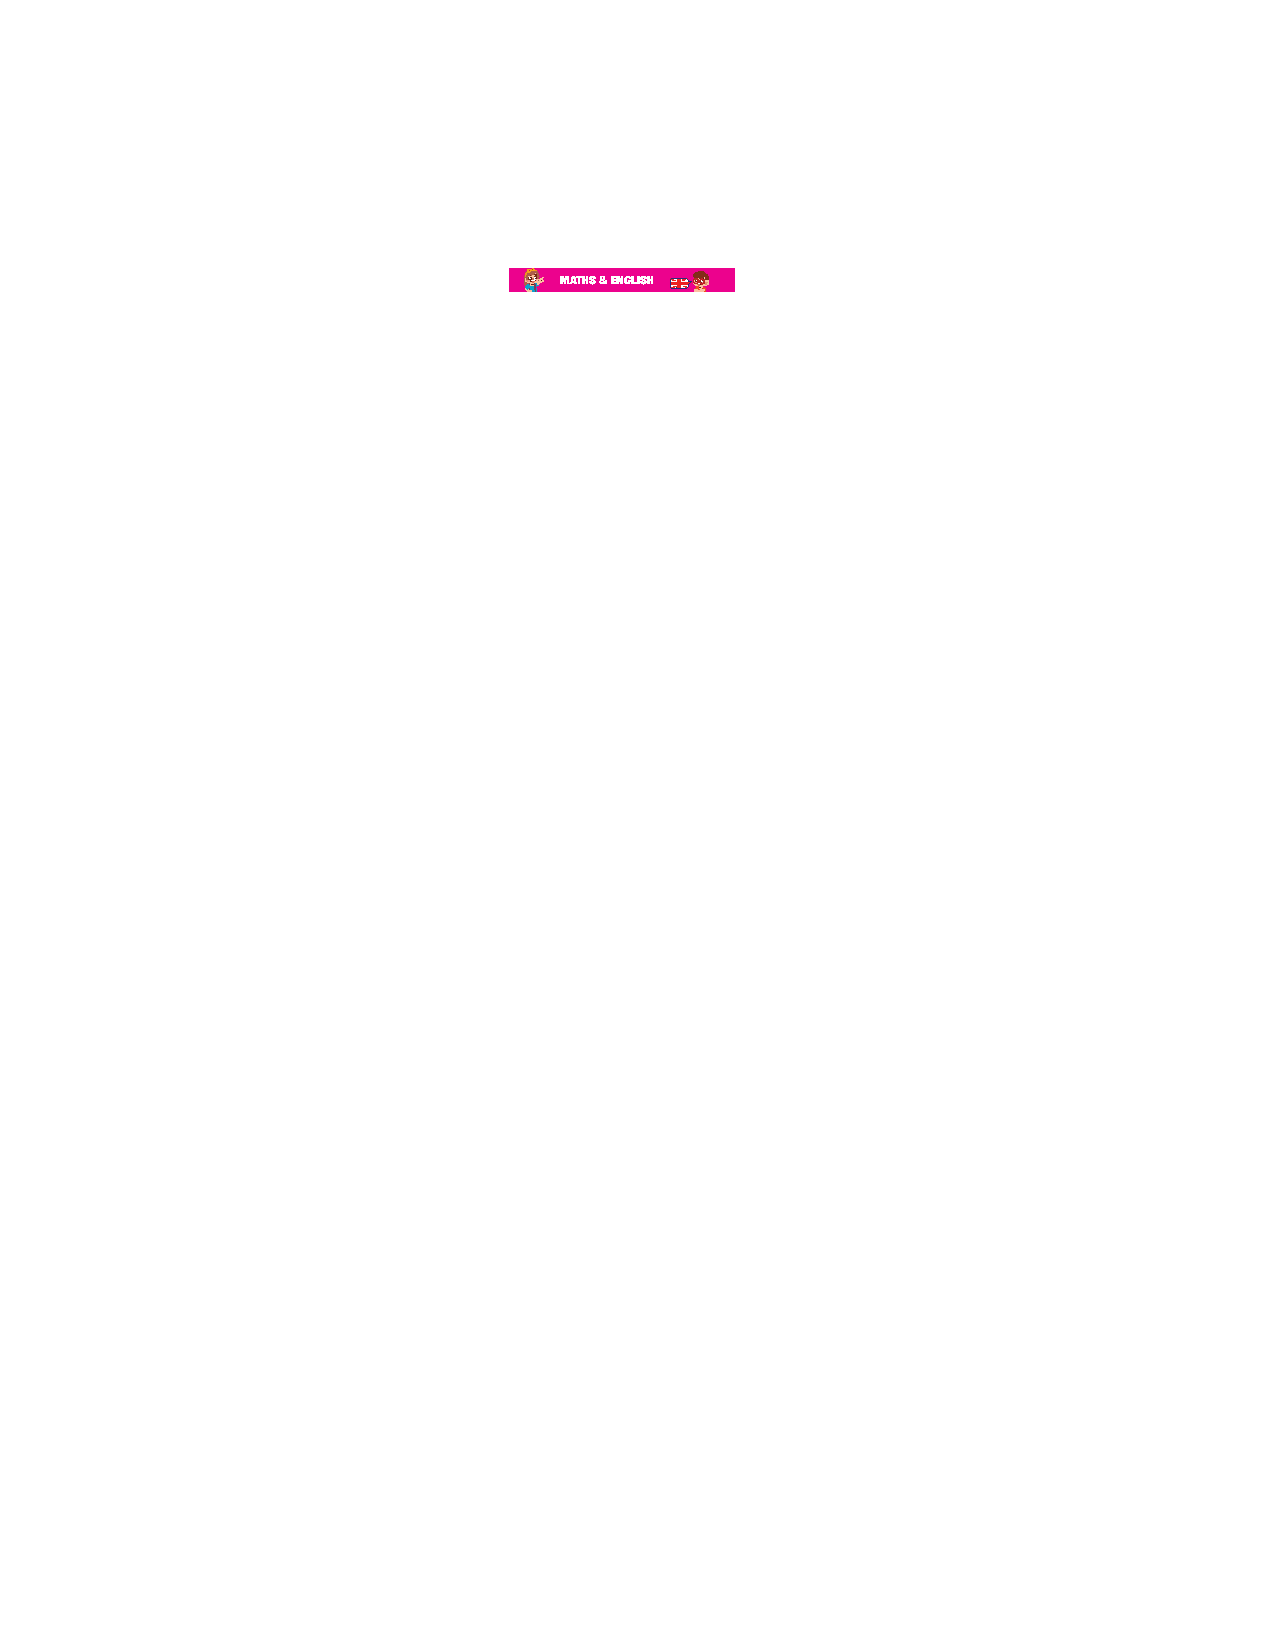
\includegraphics[width=17.2cm]{../mathc.pdf}}}
%\AddToShipoutPicture*{\put(-2,733){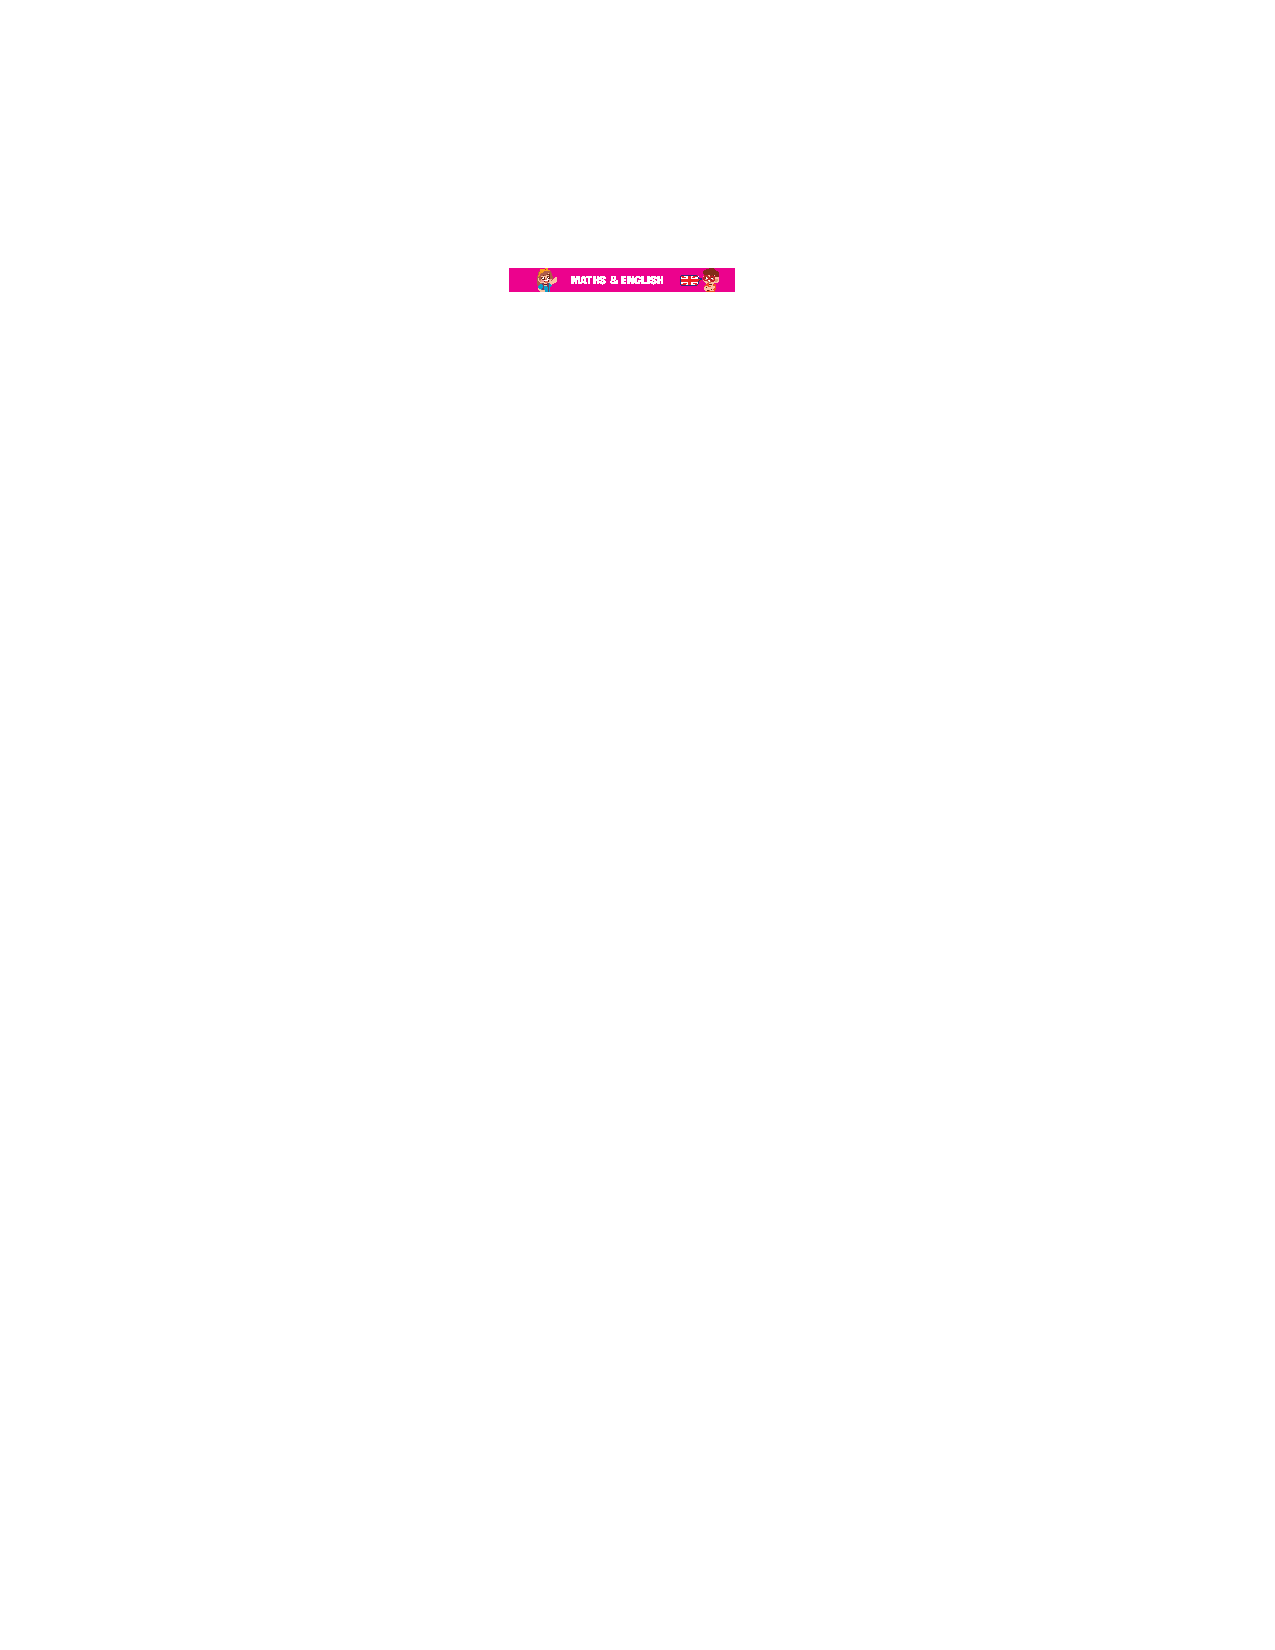
\includegraphics[width=17.2cm]{../mathl.pdf}}} 
\AddToShipoutPicture*{\put(112,675){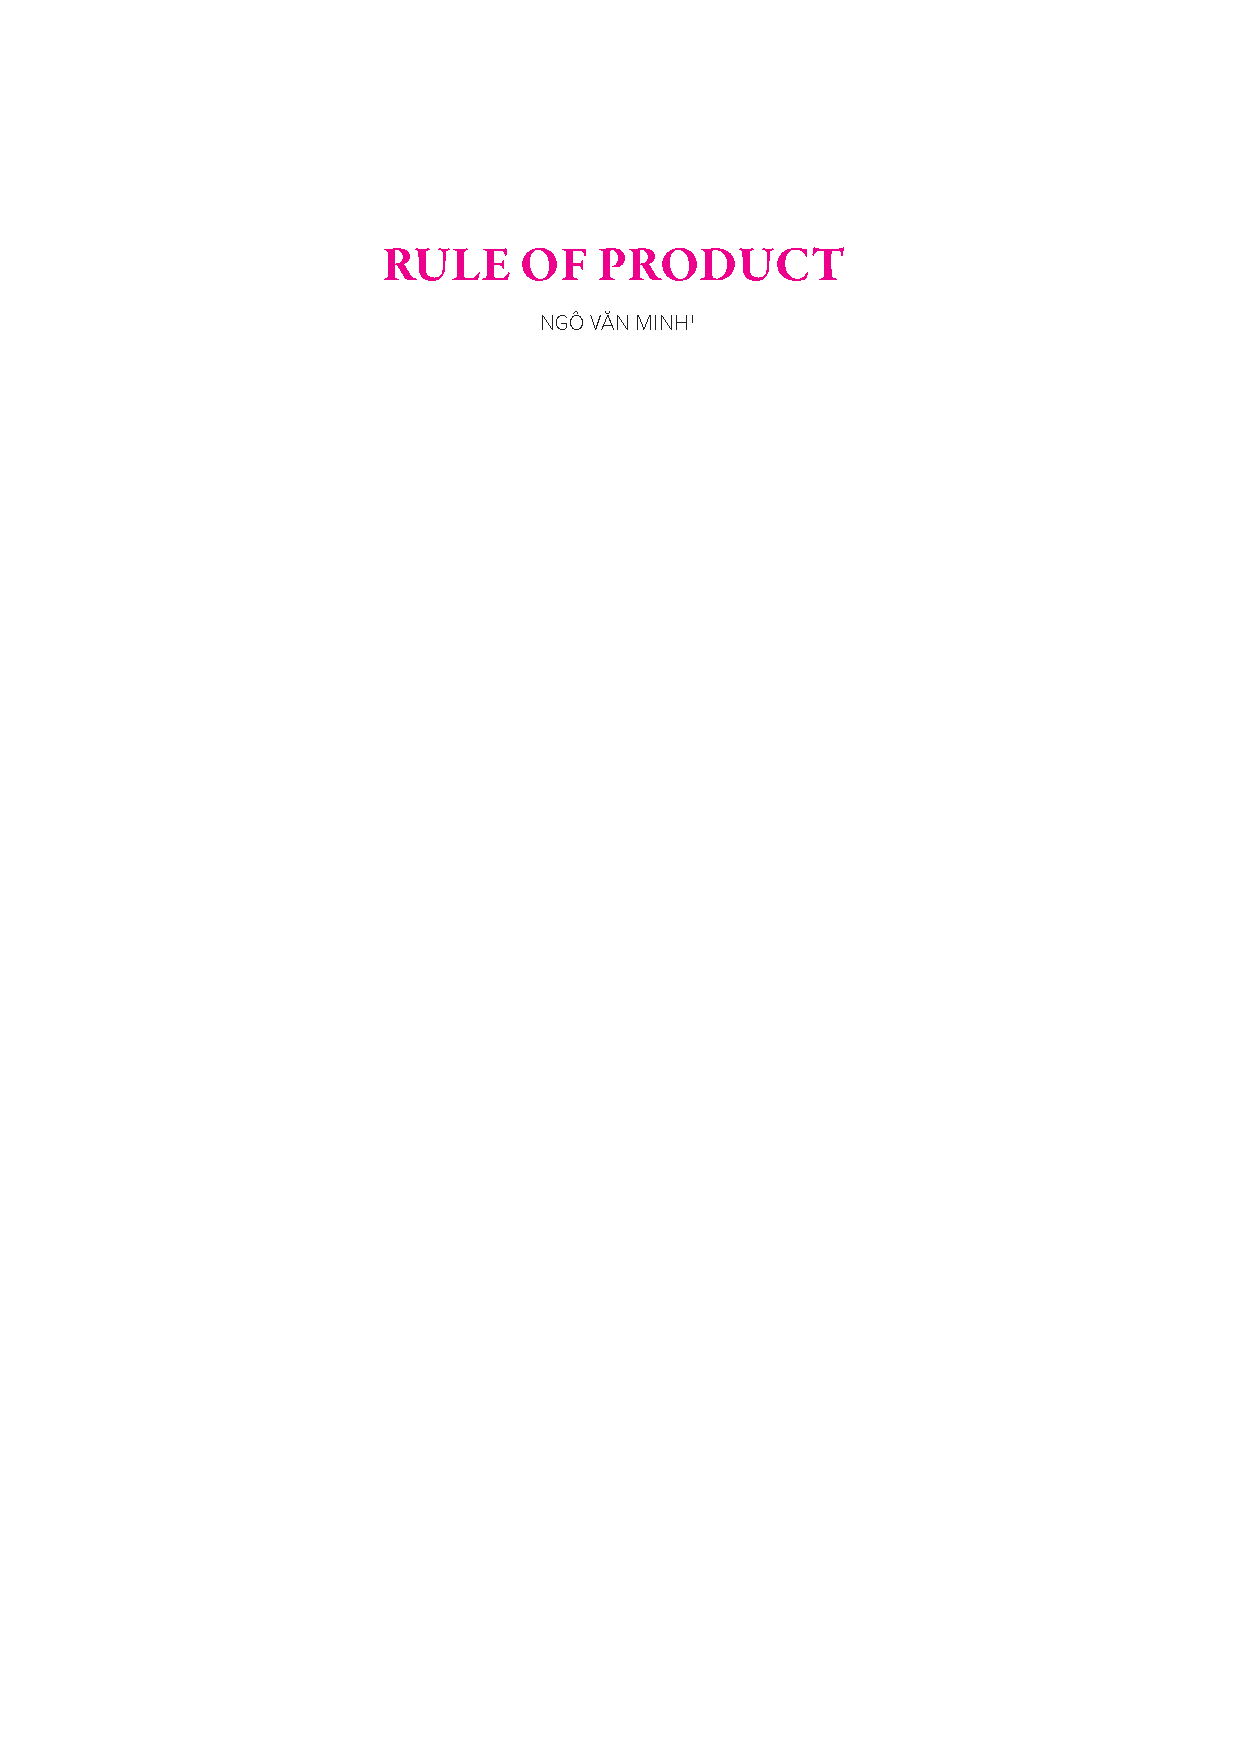
\includegraphics[scale=1]{../tieude3.pdf}}} 
\centering
\endgroup
\graphicspath{{../toancuabi/pic/}}
\vspace*{35pt}

\begin{multicols}{2}
	\PIbox{\textbf{\color{toancuabi}Problem} $\pmb{1.}$ How many ways are there to color the regions $A$, $B$, $C$, $D$ in the figure with three different colors, where each region is colored by one color?}	 
	\begin{figure}[H]
		\centering
		\vspace*{-5pt}
		\captionsetup{labelformat= empty, justification=centering}
		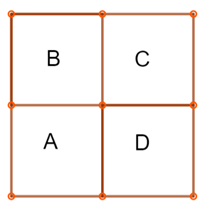
\includegraphics[scale=1]{m1}
		\vspace*{-5pt}
	\end{figure}
	\PIbox{\textbf{\color{toancuabi}Rule of Multiplication:} Suppose that we have to do two independent jobs $A$ and $B$, and that there are $m$ ways to do job $A$ and $n$ ways to do job $B$. We cannot do both jobs at the same time, then there are $(m \times n)$ ways to do \textbf{\color{toancuabi}both} jobs.}
	\vskip 0.1cm
	\textit{Solution}: There are $4$ regions to be colored, and there are $3$ ways to color each region. Therefore, the number of colorings is 
	\begin{align*}
		\text{Rule of multiplication: }	3 \times 3\times 3\times 3=81.
	\end{align*}
	\PIbox{\textbf{\color{toancuabi}Problem} $\pmb{2.}$ How many ways are there to color the regions $A$, $B$, $C$, $D$, $E$ in the figure using three different colors such that two adjacent regions have different colors?	} 
	\begin{figure}[H]
		\centering
		\vspace*{-5pt}
		\captionsetup{labelformat= empty, justification=centering}
		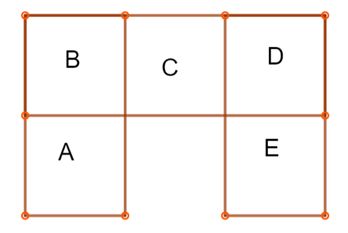
\includegraphics[scale=1]{m2}
		\vspace*{-10pt}
	\end{figure}
	\textit{Solution}: We color in the order $A \to B \to C \to D \to E$. There are $3$ ways to color region $A$. After that, there are $2$ ways to color $B$ with a different color. Then there are $2$ ways to color $C$ with a color different from $B$, and so on ...
	\vskip 0.1cm   
	According to the rule of multiplication, the number of colorings is given by
	\begin{align*}
		\text{Rule of multiplication: } 3 \times 2^4= 48.
	\end{align*}
	\PIbox{\textbf{\color{toancuabi}Problem} $\pmb{3.}$ How many ways are there to put $8$ rooks on a chessboard so that they do not attack each other? 
	\vskip 0.1cm
	(\textit{Note that two rooks on the same row or column attack each other.})}
	\begin{figure}[H]
		\centering
%		\vspace*{-5pt}
		\captionsetup{labelformat= empty, justification=centering}
		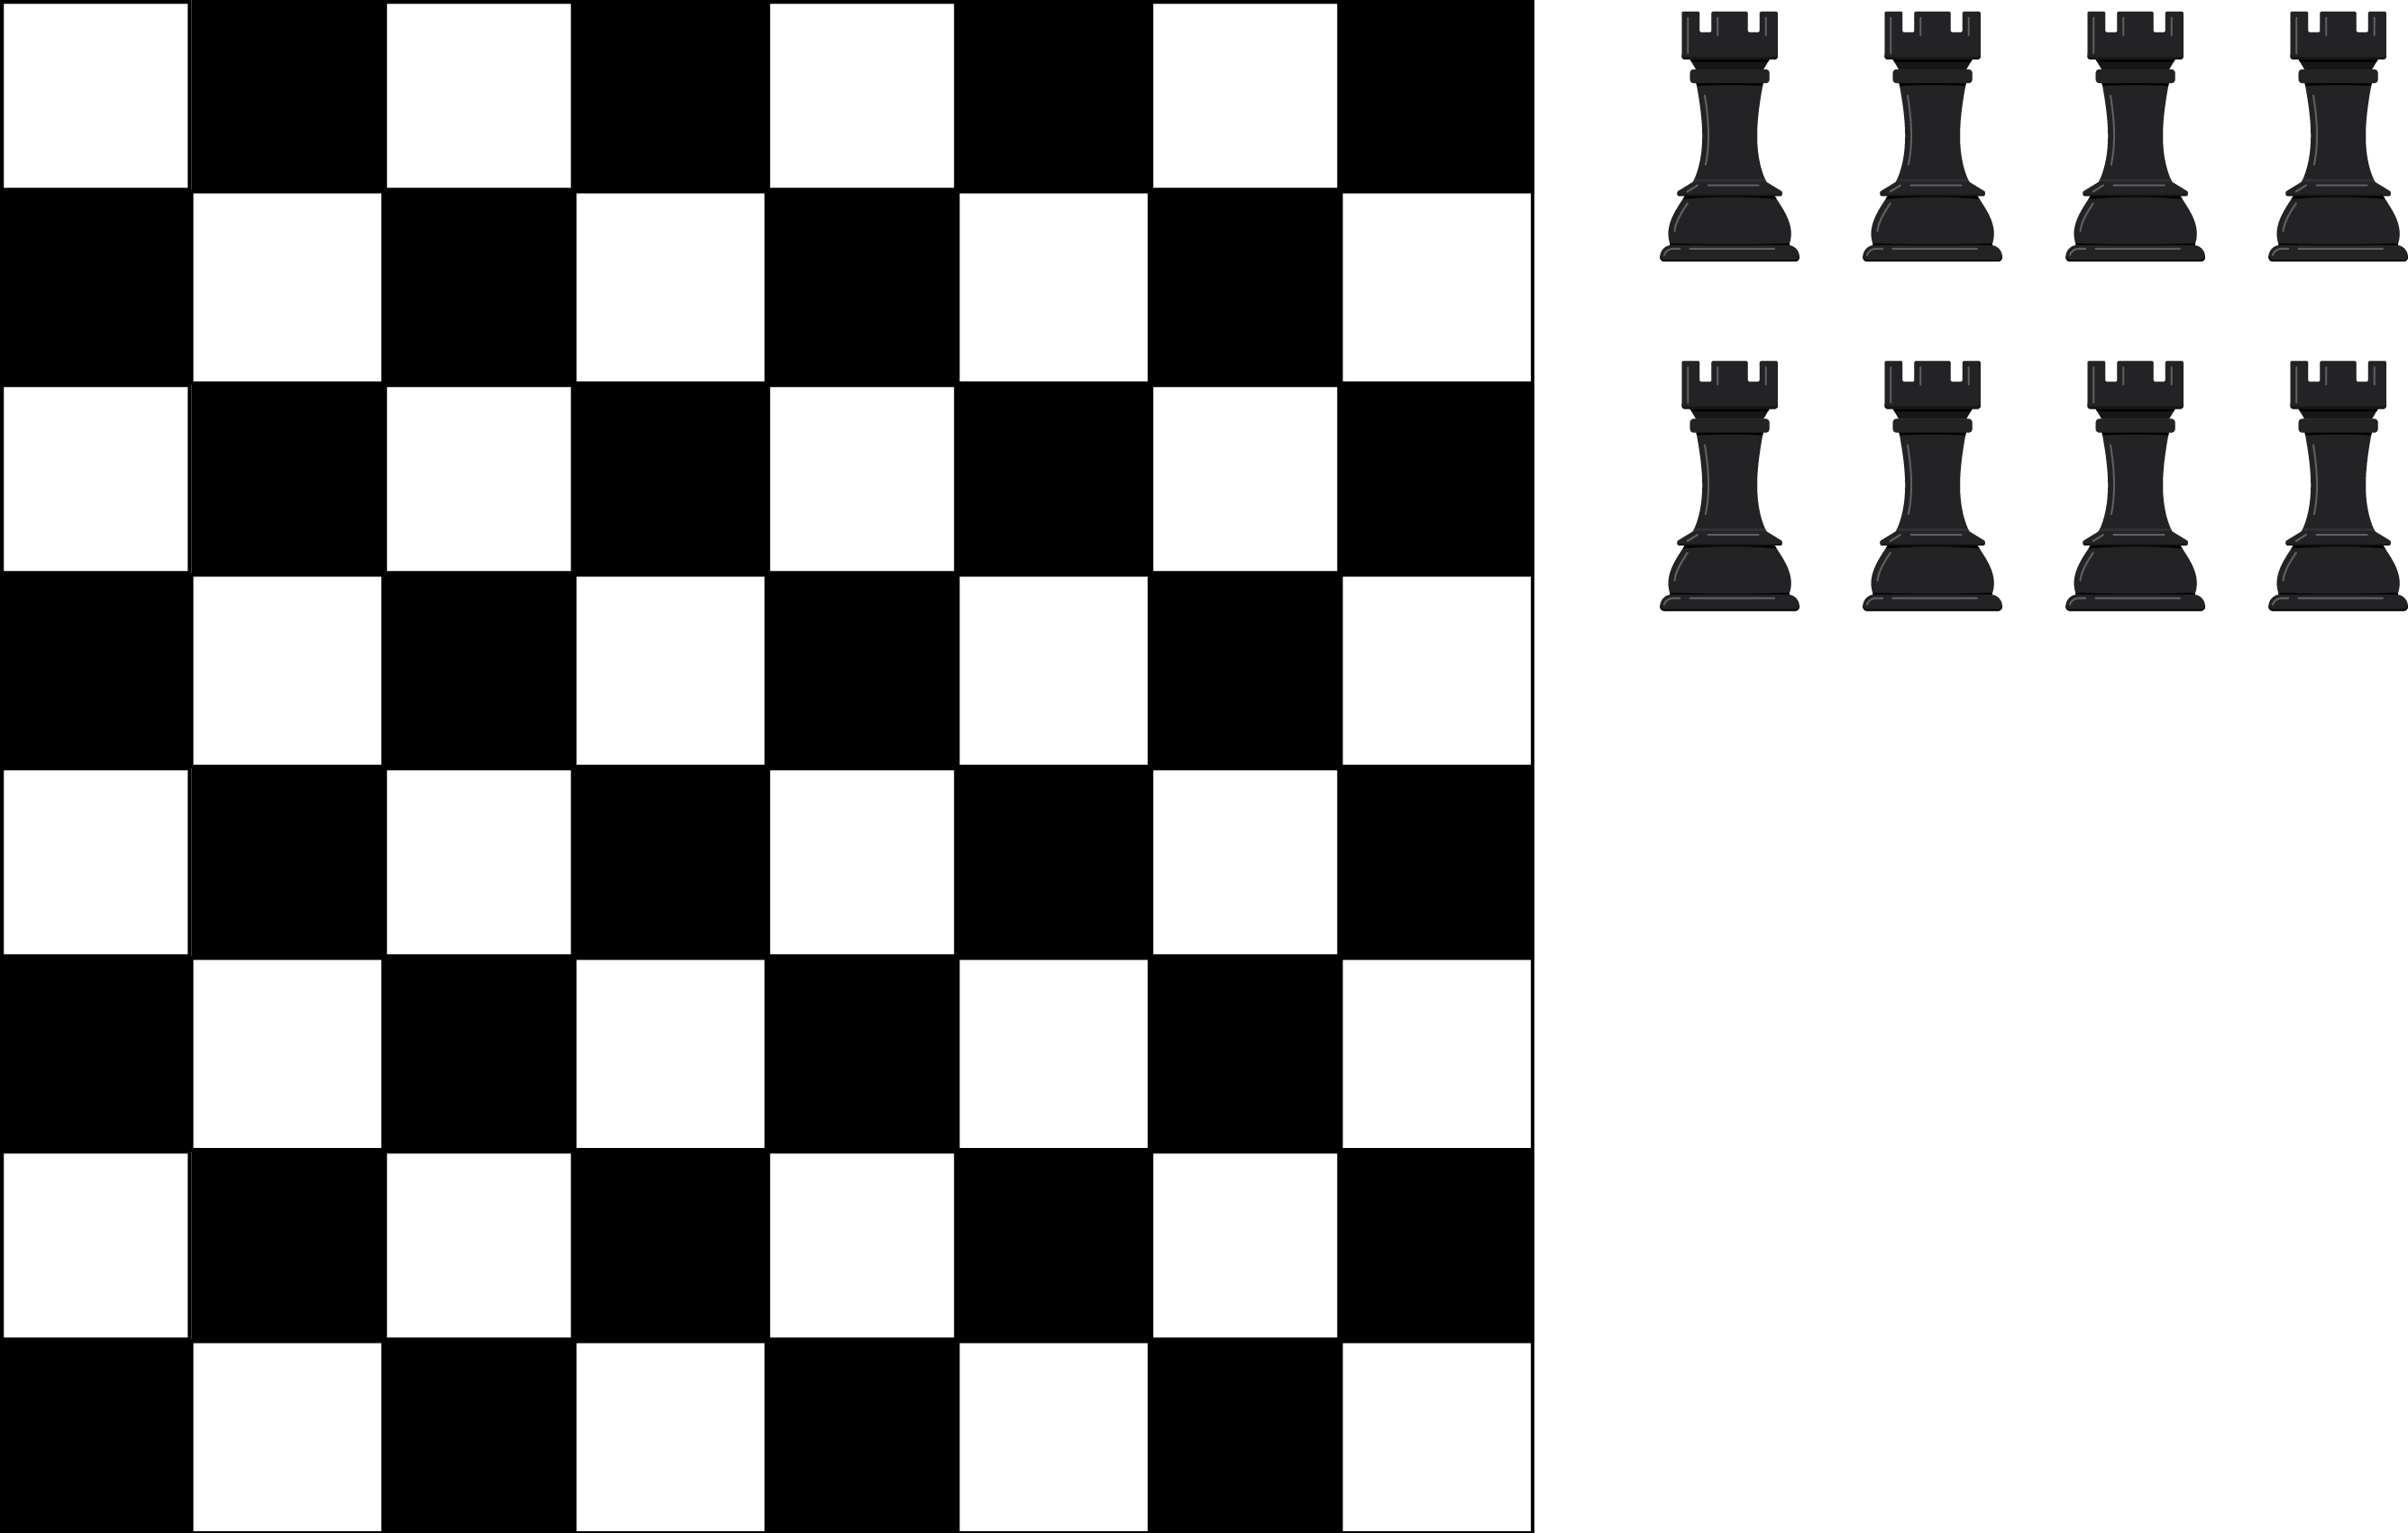
\includegraphics[width=1\linewidth]{co}
		\vspace*{-10pt}
	\end{figure}
	\textit{Solution}:
	\vskip 0.1cm 
	$\circ$ Step $1$: Put the $1^{\text{st}}$ rook on the $1^{\text{st}}$ row: $8$ ways
	\vskip 0.1cm
	$\circ$ Step $2$: Put the $2^{\text{nd}}$ rook on the $2^{\text{nd}}$ row: $7$ ways
	\vskip 0.1cm
	$\circ$ $\ldots$
	\vskip 0.1cm
	$\circ$ Step $8$: Put the $8^{\text{th}}$ rook on the $8^{\text{th}}$ row: $1$ way
	\vskip 0.1cm
	By the rule of multiplication, there are 
	\begin{align*}
		8\times7\times6\times\ldots\times1=40320
	\end{align*}
	ways to put $8$ rooks on a chessboard such that they do not attack each other.
	\vskip 0.1cm
	\PIbox{\textbf{\color{toancuabi}Problem} $\pmb{4.}$ There are $5$ {\color{green}green balls} numbered from $1$ to $5$, $6$ {\color{red}red balls} numbered from $1$ to $6$, and $7$ {\color{yellow}yellow balls} numbered from $1$ to $7$. How many ways are there to choose $3$ balls such that they have different colors and numbers?}
	\begin{figure}[H]
		\centering
		\vspace*{-5pt}
		\captionsetup{labelformat= empty, justification=centering}
		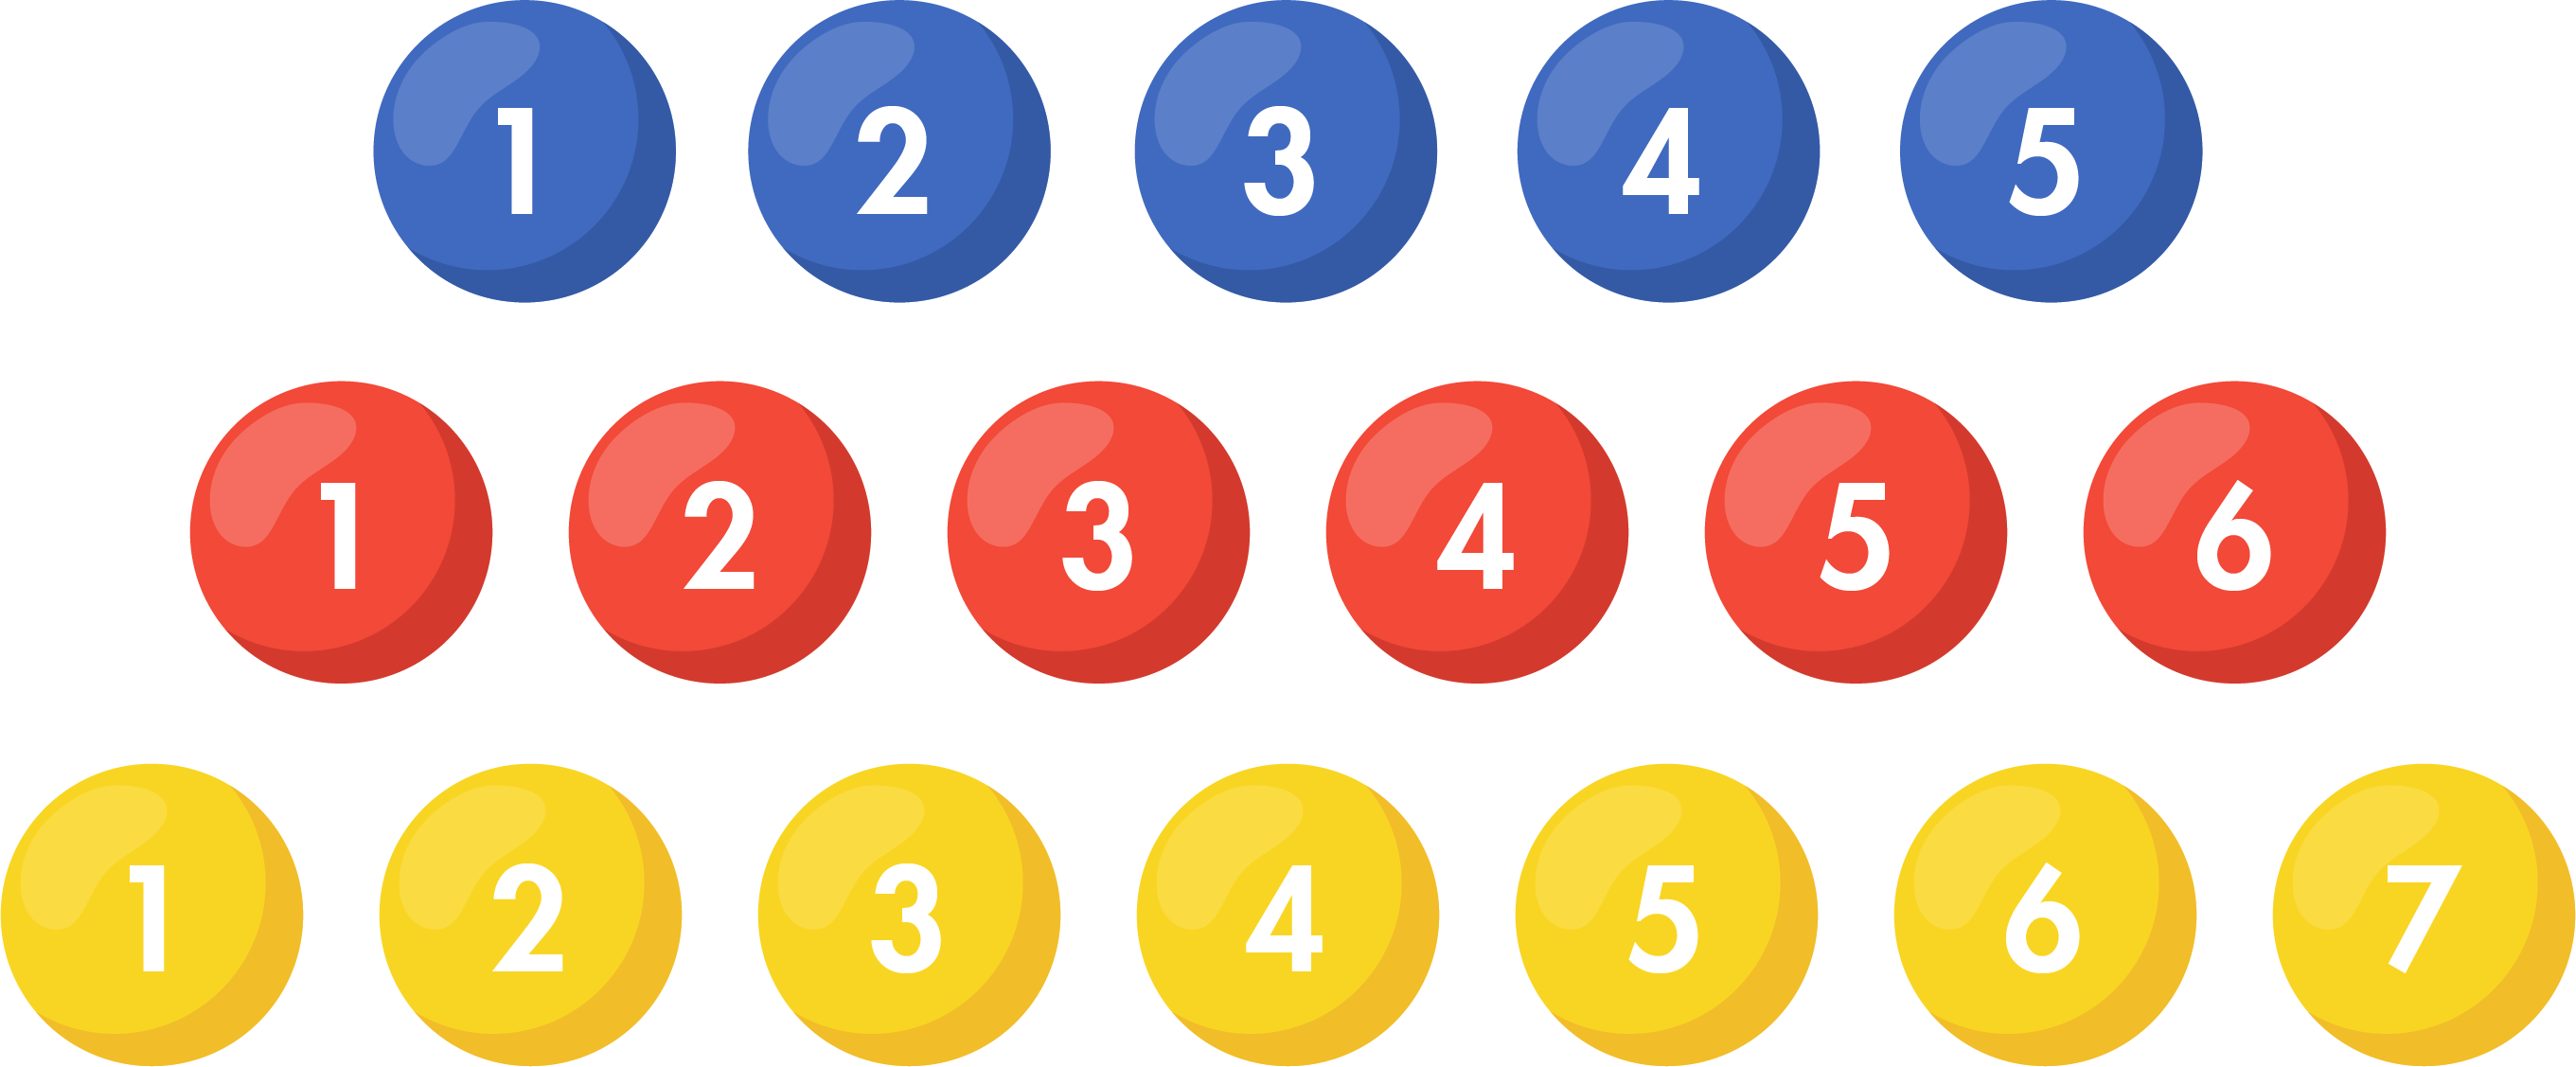
\includegraphics[width=1\linewidth]{bong}
		\vspace*{-10pt}
	\end{figure}
	\textit{Solution:}
	\vskip 0.1cm 
	$\circ$ First, we choose a {\color{green}green ball}. There are $5$ available choices. 
	\vskip 0.1cm
	$\circ$ Next, we choose a {\color{red}red ball}. The number on this {\color{red}red ball} is different from that of the {\color{green}green ball}, so there are $6-1=5$ available choices. 
	\vskip 0.1cm
	$\circ$ Finally, we choose a {\color{yellow}yellow ball}, and there are $7-2=5$ available choices. 
	\vskip 0.1cm
	According to the rule of multiplication, the number of ways to choose $3$ balls of different colors and different numbers is: 
	\begin{align*}
		5\times5\times5=125.
	\end{align*}
	\PIbox{\textbf{\color{toancuabi}Problem} $\pmb{5.}$ How many even $4$--digit numbers with distinct digits are there?}
	\vskip 0.1cm
	\textit{Solution}:  Let’s write an even $4$--digit number as $\overline{abcd}$ where $a\ne 0$, the $4$ digits $a$, $b$, $c$, $d$ are pairwise distinct, and $d$ is in the set $\{0,2,4,6,8\}$.
	\vskip 0.1cm
	We consider two cases:
	\vskip 0.1cm
	\textit{Case} $1$: $d=0$. There are $9$ ways to choose $a$, then $8$ ways to choose $b$ and then $7$ ways to choose $c$. Therefore, there are $1\times 9\times8\times7$ choices of the number $\overline{abcd}$.
	\vskip 0.1cm
	\textit{Case} $2$: $d\ne0$. There are $4$ ways to choose $d$. For each choice of $d$, there are $8$ ways to choose $a$ ($a\ne0$ and $a\ne d$), then $8$ ways to choose $b$ and then $7$ ways to choose $c$. Therefore, there are $4
	\times8\times8\times7$ choices of the number $\overline{abcd}$.
	\vskip 0.1cm
	Thus, there are 
	\begin{align*}
		1\times9\times8\times7+4\times8\times8\times7 = 2296
	\end{align*}
	numbers that satisfy the requirement of the problem.
	\vskip 0.1cm
	\PIbox{\textbf{\color{toancuabi}Exercise} $\pmb{1.}$ How many ways are there to color the regions $A$, $B$, $C$, $D$ in the figure with one color for each region, given that there are three different colors and no two adjacent regions have the same color?}
	\begin{figure}[H]
		\centering
		\vspace*{-5pt}
		\captionsetup{labelformat= empty, justification=centering}
		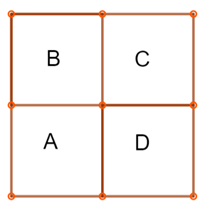
\includegraphics[scale=1]{m3}
		\vspace*{-5pt}
	\end{figure}
	\vskip 0.1cm
	\PIbox{\textbf{\color{toancuabi}Exercise} $\pmb{2.}$ How many ways are there to color the sides of a pentagon with three different colors such that no two adjacent sides have the same color?}
	\vskip 0.2cm
	\PIbox{{\centerline{\textbf{\color{toancuabi}New words}}}
		\vskip 0.2cm
		{\color{toancuabi}Adjacent(adj):} bên cạnh, cạnh nhau
		\vskip 0.1cm
		{\color{toancuabi}Case:} trường hợp 
		\vskip 0.1cm
		{\color{toancuabi}Color (v):} tô màu 
		\vskip 0.1cm
		{\color{toancuabi}Different:} khác 
		\vskip 0.1cm
		{\color{toancuabi}Region:} vùng, miền
		\vskip 0.1cm
		{\color{toancuabi}Rook (Chess):} quân Xe trên bàn cờ Vua  
		\vskip 0.1cm
		{\color{toancuabi}Rule of Multiplication:} Quy tắc Nhân
		\vskip 0.1cm
		{\color{toancuabi}Way:} con đường, cách (thực hiện) }
\end{multicols}